\documentclass[12pt,openright,twoside,a4paper,english,french,spanish]{abntex2}

\usepackage{cmap}	
\usepackage{lmodern}	
\usepackage[T1]{fontenc}	
\usepackage[utf8]{inputenc}		
\usepackage{lastpage}		
\usepackage{indentfirst}
\usepackage{color}	
\usepackage{graphicx}	
\usepackage{units}
\usepackage[brazilian,hyperpageref]{backref}
% \usepackage[alf]{abntex2cite}
\usepackage{bold-extra}
\usepackage{eso-pic}
%
\usepackage{tikz}
% \usepackage[]{circuitikz}
\usepackage[american,cuteinductors,smartlabels]{circuitikz}

\usepackage{lipsum}
\usepackage{listings}
\usepackage{caption}
% \usepackage[acronym]{glossaries} 
\usepackage[subentrycounter,seeautonumberlist,nonumberlist=true]{glossaries}
\usepackage[brazilian,hyperpageref]{backref}	 % Paginas com as citações na bibl
\usepackage[alf]{abntex2cite}	% Citações padrão ABNT
\usepackage{subcaption}
\usepackage{multicol}
\usepackage{multirow}

\renewcommand{\backrefpagesname}{Citado na(s) página(s):~}
\renewcommand{\backref}{}
\renewcommand*{\backrefalt}[4]{
	\ifcase #1 %
		Nenhuma citação no texto.%
	\or
		Citado na página #2.%
	\else
		Citado #1 vezes nas páginas #2.%
	\fi}%
% ---


\newcommand{\curso}[1]{\def\imprimircurso{#1}}

\newcommand{\palavraChaveUm}[1]{\def\imprimirpalavrachaveum{#1}}
\newcommand{\palavraChaveDois}[1]{\def\imprimirpalavrachavedois{#1}}

\newcommand{\cdu}[1]{\def\nomecdu{#1}}
\newcommand{\dataDaAprovacao}[1]{\def\imprimirdatadaaprovacao{#1}}

\newcommand{\membroConvidadoUm}[1]{\def\imprimirmembroconvidadoum{#1}}
\newcommand{\membroConvidadoDois}[1]{\def\imprimirmembroconvidadodois{#1}}

\newcommand\BackgroundPic{%
	\put(0,0){%
		\parbox[b][\paperheight]{\paperwidth}{%
			\vfill
			\centering
			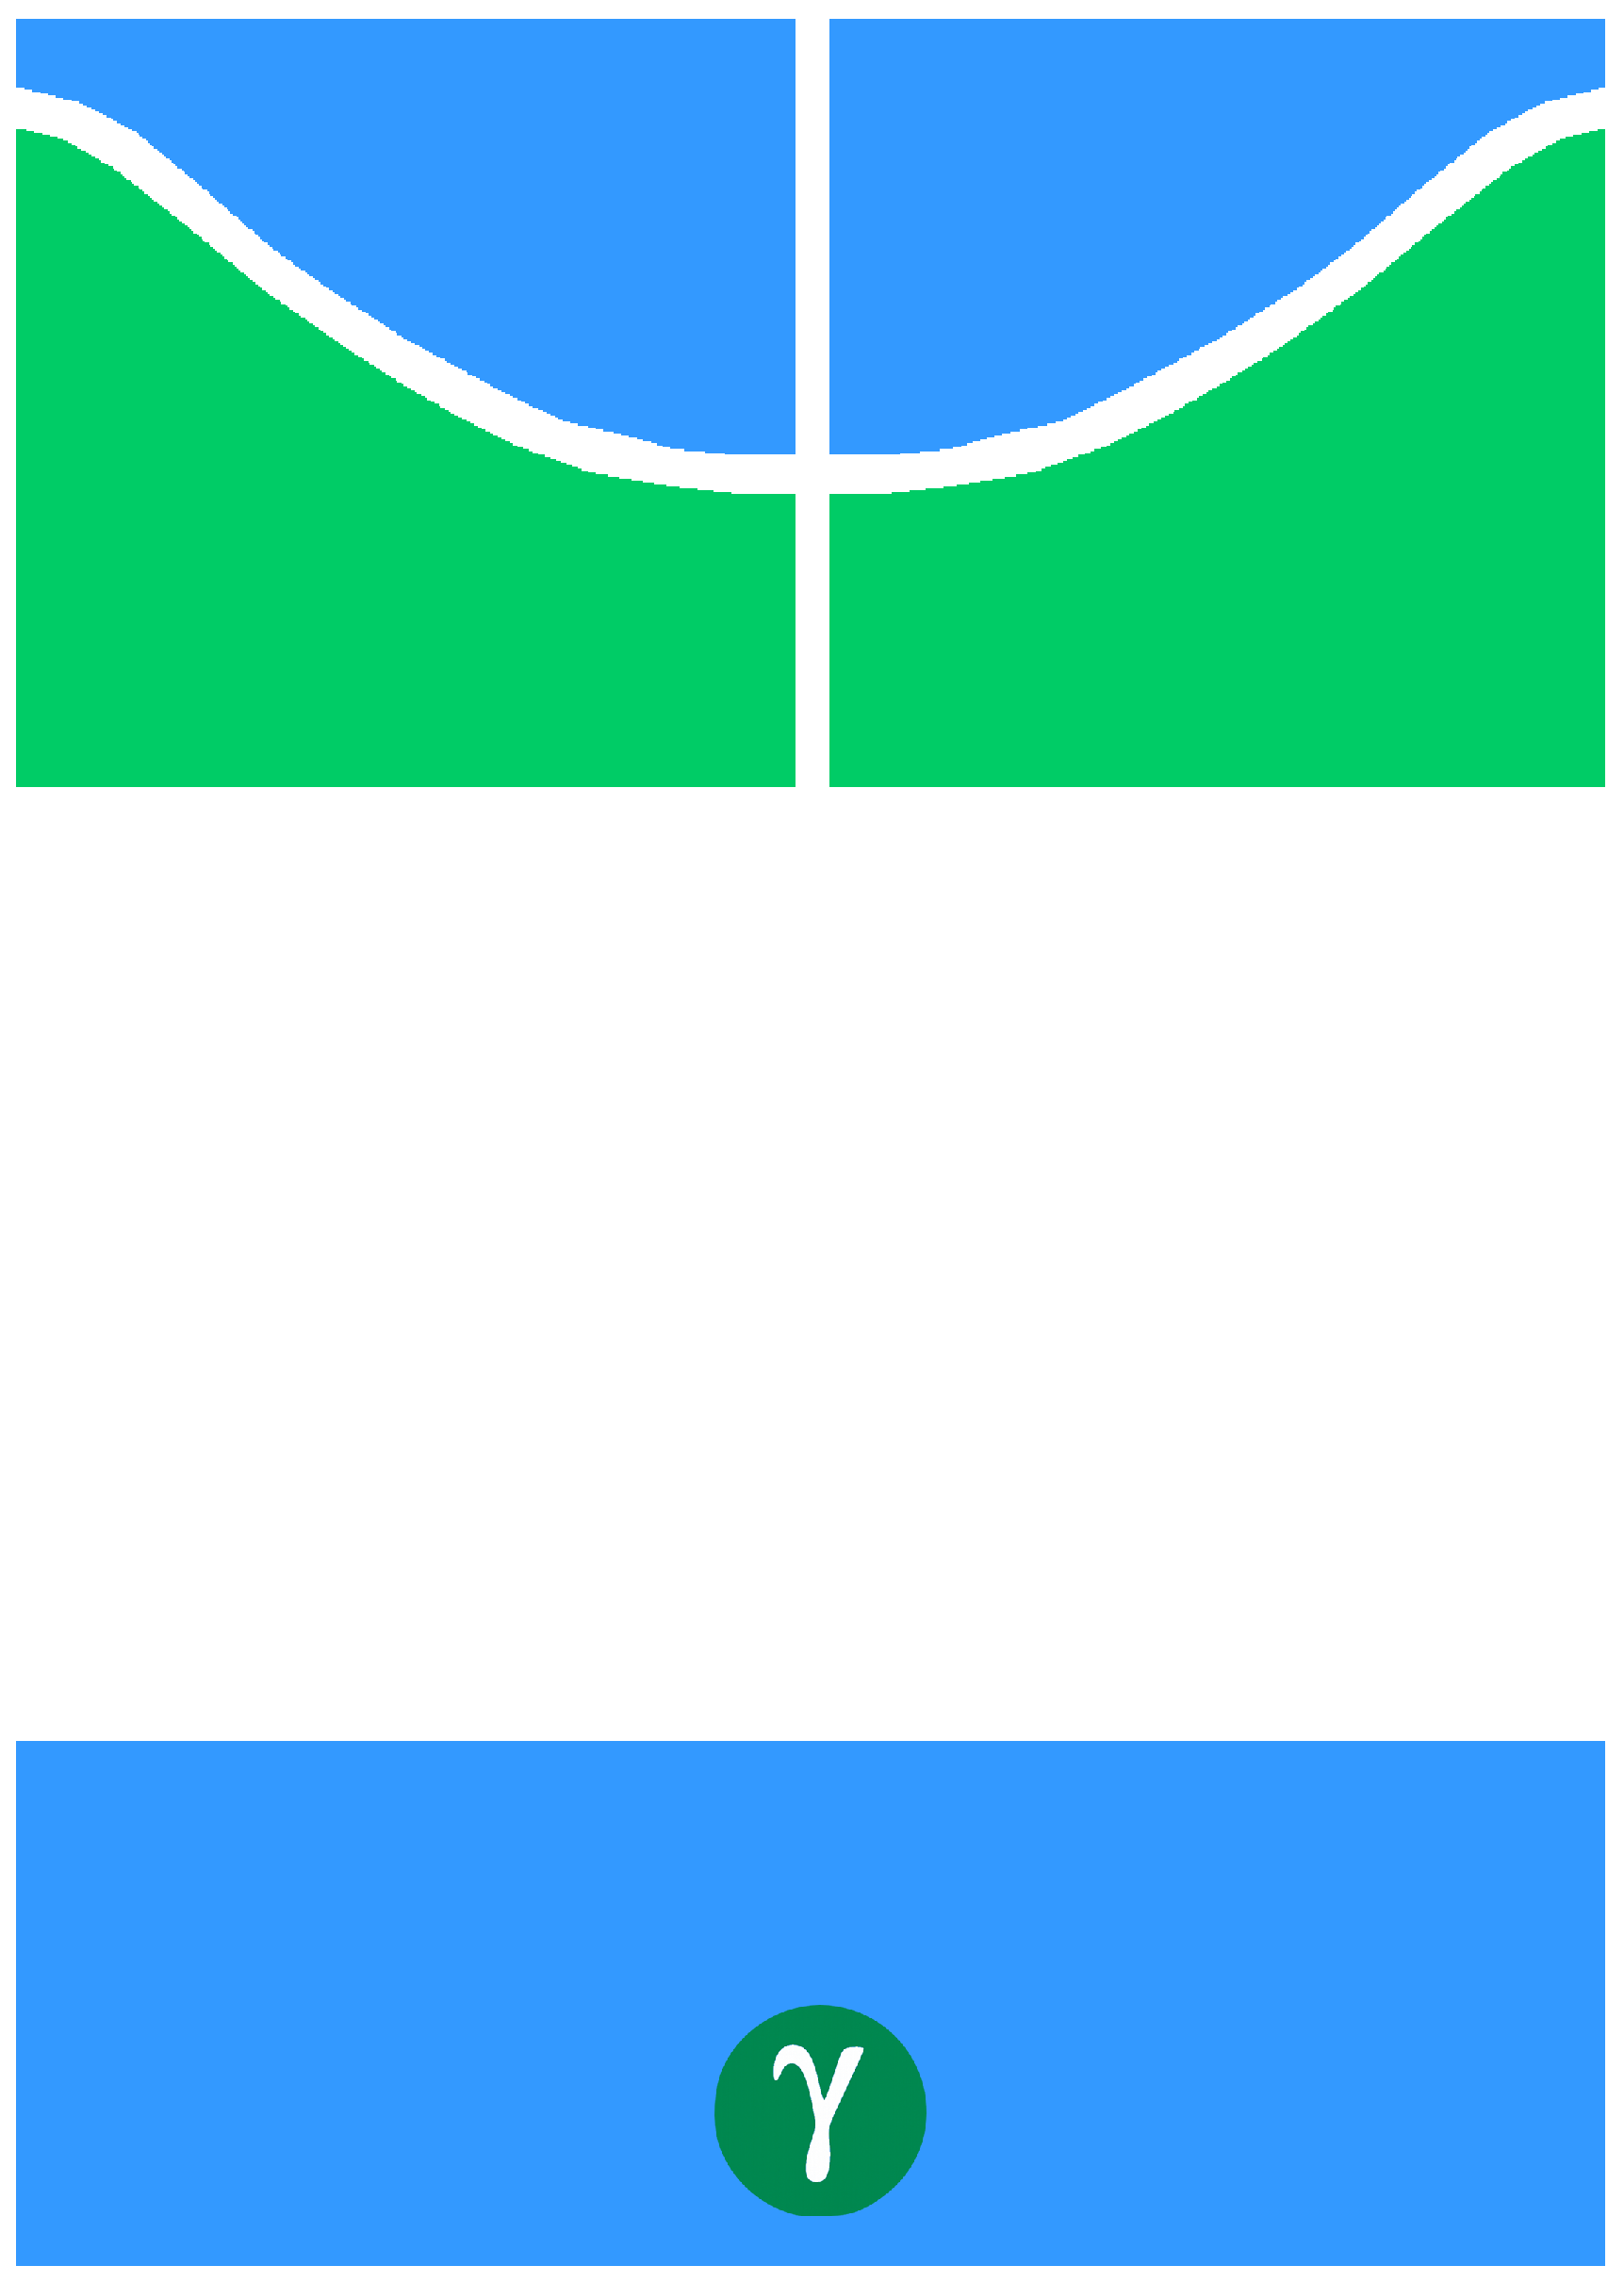
\includegraphics[width=\paperwidth,height=\paperheight,%
				keepaspectratio]{figuras/capa.eps}%
			\vfill
		}
	}
}

\renewcommand{\imprimircapa}{%
  \begin{capa}%
    \center
	\AddToShipoutPicture*{\BackgroundPic}

%	\begin{huge}
%		\textbf{\textsc{Trabalho de Conclusão de Curso}}
%	\end{huge}

    \vspace*{2.7in}
	{\textbf{\large\imprimirinstituicao}}
	\par
	{\textbf{\large\imprimircurso}}

	\vspace{0.5in}

    {\ABNTEXchapterfont\bfseries\HUGE\imprimirtitulo}
    \vspace*{\fill}
    
	\begin{flushright}
    	\textbf{{\large{ \imprimirautor}}}
		\par
    	\textbf{{\large{ \imprimirorientador}}}
	\end{flushright}
		
    \vspace*{0.2in}
    \textbf{{\large\imprimirlocal}}
    \par
    \textbf{{\large\imprimirdata}}
    
    \vspace*{2.2in}
  \end{capa}
}



% Dados pessoais
\autor{}
\curso{}

% Dados do trabalho
\titulo{Posicionador de Lente}
\data{14 de maio 2014}
\palavraChaveUm{contratos}
\palavraChaveDois{ágeis}


% Dados da orientacao
\orientador{}
\coorientador{(quando houver, Titulação Acadêmica e Nome do Orientador)}

% Dados para a ficha catalográfica
\cdu{02:141:005.6}

% Dados da aprovação do trabalho
\dataDaAprovacao{01 de junho de 2013}
\membroConvidadoUm{Titulação e Nome do Professor Convidado 01}
\membroConvidadoDois{Titulação e Nome do Professor Convidado 02}

\local{Brasília, DF}
\instituicao{%
  Universidade de Brasília - UnB
  \par
  Faculdade UnB Gama - FGA
}
\tipotrabalho{}

\definecolor{blue}{RGB}{41,5,195}
\makeatletter
\hypersetup{
     	%pagebackref=true,
		pdftitle={\@title}, 
		pdfauthor={\@author},
    	pdfsubject={Bike-X},
	    pdfcreator={LaTeX with abnTeX2},
		pdfkeywords={Rift, }{Unity 3D, }{abntex, }{Sensores Fisiol\'ogicos, }{Ambiente Virtual}, 
		colorlinks=true,       		% false: boxed links; true: colored links
    	linkcolor=blue,          	% color of internal links
    	citecolor=blue,        		% color of links to bibliography
    	filecolor=magenta,      		% color of file links
		urlcolor=blue,
		bookmarksdepth=4
}
\makeatother
\setlength{\parindent}{1.3cm}
\setlength{\parskip}{0.2cm}  
\makeindex

\usetikzlibrary{shapes,arrows,shadows}
\usetikzlibrary{mindmap,trees}
\usetikzlibrary{calc,decorations.pathmorphing,patterns}
\pgfdeclaredecoration{penciline}{initial}{
    \state{initial}[width=+\pgfdecoratedinputsegmentremainingdistance,
    auto corner on length=1mm,]{
        \pgfpathcurveto%
        {% From
            \pgfqpoint{\pgfdecoratedinputsegmentremainingdistance}
                      {\pgfdecorationsegmentamplitude}
        }
        {%  Control 1
        \pgfmathrand
        \pgfpointadd{\pgfqpoint{\pgfdecoratedinputsegmentremainingdistance}{0pt}}
                    {\pgfqpoint{-\pgfdecorationsegmentaspect
                     \pgfdecoratedinputsegmentremainingdistance}%
                               {\pgfmathresult\pgfdecorationsegmentamplitude}
                    }
        }
        {%TO 
        \pgfpointadd{\pgfpointdecoratedinputsegmentlast}{\pgfpoint{1pt}{1pt}}
        }
    }
    \state{final}{}
}


% \usepackage{tikzgraphicx}

\tikzstyle{cloud} = [draw, ellipse,fill=blue!20, node distance=3cm,
    minimum height=3em]
\tikzstyle{estado} = [draw, ellipse,fill=blue!20, node distance=3cm,align=center]
\tikzstyle{teste} = [draw, diamond,fill=green!20, node distance=3cm,align=left]
%    minimum height=2em]
\tikzstyle{ciclo} =[draw, rectangle,fill=blue!20, node distance=3cm,align=center,decorate,thick,minimum height=3em]
\tikzstyle{phanton} = []   
\tikzstyle{line} = [->,right] %[draw, -latex']
\tikzstyle{retorno} = [loop above]
\tikzstyle{arrow} = [bend left,->]
\tikzset{
    %Define standard arrow tip
    >=stealth',
    %Define style for boxes
    punkt/.style={
           rectangle,
           rounded corners,
           draw=black, very thick,
           text width=6.5em,
           minimum height=2em,
           text centered},
    % Define arrow style
    pil/.style={
           ->,
           thick,
           shorten <=2pt,
           shorten >=2pt,}
}
\newglossaryentry{rift}
{
	name = Oculus Rift,
	text = \textit{Oculus Rift},
	description={Equipamento de realidade virtual para jogos eletrônicos}
}

\newglossaryentry{msp}
{
	name = MSP430,
	text = \textit{MSP430},
	description={Microcontrolador de baixa potência da Texas Instruments (TI). A versão utilizada neste projeto é a MSP430G2553, disponibilizada junto ao kit \href{http://www.ti.com/tool/msp-exp430g2}{Launchpad}}
}

\newglossaryentry{rs232}
{
	name = UART (RS232),
	text = \textit{UART},
	description={Padrão de protocolo para troca serial de dados binários entre um DTE (terminal de dados) e um DCE(comunicador de dados). Também é conhecido por \textit{EIA RS-232C} ou \textit{V.24)}}
}

\newglossaryentry{python}
{
	name = Python,
	text = \textit{Python},
	description={Python é uma linguagem de programação de alto nível , interpretada, imperativa, orientada a objetos, funcional, de tipagem dinâmica e forte. Foi lançada por Guido van Rossum em 1991\cite{python_history}. Atualmente possui um modelo de desenvolvimento comunitário, aberto e gerenciado pela organização sem fins lucrativos Python Software Foundation}
}
\makeglossaries

\begin{document}

\frenchspacing 
\imprimircapa
\imprimirfolhaderosto*

\begin{center}

\chapter*{Equipe}

Camila Ferreira \\
\textbf{Charles Daniel} \\
Gabriela Navarro \\
José Alberto \\
José Alisson \\
Julio Cezar do Nascimento \\
Lucas Kanashiro \\
Luiz Fernando Gomes de Oliveira \\
Macartur Sousa \\
Priscila Pires \\
Tatiana Dias \\
Thiago Ferreira Gomes

\vspace{3cm}

\let\clearpage\relax
\chapter*{Professores Coordenadores}

Alessandro Borges de Sousa Oliveira \\
Edson Mintsu Hung \\
Juliana Petrocchi Rodrigues \\
Ricardo Ajax Dias Kosloski \\
Ricardo Matos Chaim  \\
Suélia de Siqueira Rodrigues Fleury Rosa 

\end{center}

\newpage

% \begin{fichacatalografica}
	\vspace*{\fill}					% Posição vertical
	\hrule							% Linha horizontal
	\begin{center}					% Minipage Centralizado
	\begin{minipage}[c]{12.5cm}		% Largura
	
	\imprimirautor
	
	\hspace{0.5cm} \imprimirtitulo  / \imprimirautor. --
	\imprimirlocal, \imprimirdata-
	
	\hspace{0.5cm} \pageref{LastPage} p. : il. (algumas color.) ; 30 cm.\\
	
	\hspace{0.5cm} \imprimirorientadorRotulo~\imprimirorientador\\
	
	\hspace{0.5cm}
	\parbox[t]{\textwidth}{\imprimirtipotrabalho~--~\imprimirinstituicao,
	\imprimirdata.}\\
	
	\hspace{0.5cm}
		1. \imprimirpalavrachaveum.
		2. \imprimirpalavrachavedois.
		I. \imprimirorientador.
		II. Universidade de Brasília.
		III. Faculdade UnB Gama.
		IV. \imprimirtitulo\\ 			
	
	\hspace{8.75cm} CDU \nomecdu\\
	
	\end{minipage}
	\end{center}
	\hrule
\end{fichacatalografica}

% \begin{epigrafe}
    \vspace*{\fill}
	\begin{flushright}
		\textbf{A epígrafe é opcional. Caso não deseje uma, deixe todo
		este arquivo em branco}.

		\textit{``Não vos amoldeis às estruturas deste mundo, \\
		mas transformai-vos pela renovação da mente, \\
		a fim de distinguir qual é a vontade de Deus: \\
		o que é bom, o que Lhe é agradável, o que é perfeito.\\
		(Bíblia Sagrada, Romanos 12, 2)}
	\end{flushright}
\end{epigrafe}

\pdfbookmark[0]{\contentsname}{toc}
\tableofcontents*
\cleardoublepage


\textual

\part{Escopo do produto}
\chapter[Problema]{Problema}

O estilo de vida do ser humano mudou drasticamente ao longo dos últimos séculos. Atividades que antes eram realizadas por pessoas passaram a ser executadas 
por máquinas, e sistemas eletrônicos, exigindo cada vez menos do corpo humano. Esta diminuição em atividades físicas tem levado as pessoas a tomar um estilo 
de vida mais sedentário, provocando um aumento nos índices de doenças crônicas como obesidade, diabetes, hipertensão e uma série de outras doenças. Desta forma, 
as organizações de saúde recomendam uma alimentação balanceada e principalmente a prática de exercícios físicos para combater os problemas causados pelo 
sedentarismo.

Dentre as diversas formas de atividade física, o ciclismo se destaca por ser uma atividade simples e agradável ao ciclista. O ciclismo permite ao praticante 
exercitar vários músculos do corpo e trabalhar a coordenação motora. Além disso, o contato com o ambiente torna esta prática mais prazerosa ao usuário. No 
entanto, existem diversos fatores que dificultam a prática desta atividade nas grandes cidades brasileiras.
A primeira das dificuldades enfrentadas por ciclistas é o acesso a espaços apropriados para a prática do ciclismo. A ausência de ciclovias obriga ao ciclistas 
a utilizar as ruas e a dividir espaço com motoristas, que geralmente não aceitam dividir o espaço pelo fato dos ciclistas trafegarem em velocidades menores que 
a dos carros, podendo causar acidentes. Mesmo quando há ciclovias, os ciclistas tem de enfrentar as avenidas urbanas para chegar ao local, novamente interagindo 
com motoristas.

Outros fatores que tornam a prática do ciclismo mais difícil envolvem questões relacionadas a falta de estrutura urbana. Muitas cidades brasileiras não são 
planejadas para o ciclismo, mesmo como forma de locomoção, pois quando há ciclovias, elas são geralmente descontínuas. 

Em Pelotas, Rio Grande do Sul, Brasil, \cite{barros2003}, comparando informações de boletins de ocorrência e atendimentos no pronto-socorro durante dois anos, encontraram 33,0\% de sub-registros relativos aos acidentes com lesão corporal envolvendo ciclistas.

Buracos e falta de recapeamento nas ciclovias também podem acarretar em acidentes e causar lesões aos ciclistas. Os ciclistas mais regulares afirmam também que a falta de bicicletários os obrigam a improvisar formas de fixar seu veículo. Outro fator que contribui para as dificuldades enfrentadas por ciclistas é a falta de segurança e de estrutura em espaços públicos, onde a falta de iluminação ou mesmo as abordagens de assaltantes tornam a prática mais arriscada.

Para as pessoas que não praticam atividades físicas, a principal justificativa é a falta de tempo com relação a suas atividades diárias. Em especial para o 
ciclismo, de fato, é necessário um gasto de tempo até a chegada em uma área apropriada para uma circulação mais tranquila de bicicletas. Como alternativa, as 
bicicletas ergométricas que em sua maioria estão presentes em academias são um incentivo a prática do ciclismo e devido a sua estrutura mecânica, tendem a ser 
mais confortáveis para o praticante.
Outra característica destas bicicletas é que pelo fato de serem fixas, oferecem menos riscos de lesões causadas por quedas. Além disso, o stress causado pelo 
trânsito em avenidas movimentadas não existe para este caso. Apesar de permitir simular os movimentos da pedalada de uma bicicleta comum, a bicicleta ergométrica 
tem a desvantagem de não oferecer estímulo do ambiente ao usuário. Com isso, exercitar-se em uma bicicleta ergométrica se torna uma atividade monótona ao 
praticante.



\chapter[Proposta]{Proposta}

Desejamos construir um sistema que torne a prática do exercício algo prazeroso, saudável e seguro. Para isso o sistema contará 
com a integração com realidade virtual junto com uma bicicleta real. Com o sistema de realidade virtual o usuário poderá ficar entretido enquanto 
realiza seus exercícios e poderá ter uma experiência de andar de bicicleta em um parque em sua casa ou academia, o usuário também poderá monitorar
alguns informações baseado na sua realização do exercício físico. Espera-se que o sistema esteja o mais próximo da autossuficiência energética, tornando-o mais
sustentável.

Os potenciais consumidores para o projeto são donos de academias e o usuário convencional. Donos de grandes academias estão sempre na busca de novos equipamentos mais modernos e sofisticados para atrair clientes que priorizam um ambiente diferenciado. O usuário convencional se classifica como sendo aquela pessoa que tem como \textit{hobby} andar de bicicleta ou simplesmente tem forte interesse em praticar esportes utilizando tecnologia de ponta.

\chapter[Projeto]{Projeto}
O projeto contará com diversas interações com o usuário que tem como objetivo fornecer a melhor sensação de utilizar uma bicicleta em um parque. O projeto irá ser feito de forma modular, para que a constituição final do produto seja feita com base nas necessidades de cada usuário. 

Nesse sentido, o protótipo contará com uma bicicleta e uma base que possa fixar essa bicicleta. Para dar a sensação de que o usuário estará pedalando, utilizaremos um rolo para que a roda traseira possa ser utilizada normalmente. O guidão também será utilizado de forma natural e um sensor será utilizado para definir qual a direção o usuário está virando. 

Para a realidade virtual, iremos fazer a modelagem de um ambiente e utilizando o \textit{Oculus Rift}, iremos fazer uma imersão do usuário em uma área que normalmente seria utilizada para um passeio de bicicleta. O usuário poderá ter acesso a algumas informações referentes ao seu passeio e exercício, tais como: velocidade, batimento cardíaco e outras. 

O \textit{Oculus Rift} representa hoje no mercado a ferramenta que tange a fronteira da imersão em uma realidade virtual e ao mesmo tempo a acessibilidade ao usuário. As primeiras aparições de tecnologias semelhantes de imersão virtual são datadas de 1961 pela Philco\cite{boasoverview}. Atualmente hoje há diversas opções de dispositivos que oferecem uma pervasividade especifica, tais como \textit{Cave Automatic Virtual Environm}(CAVE), \textit{Head-Mounted Displays}(HMDs) e dispositivos de entrada, tais como controles sem fio ou câmeras de rastreamento.

Uma interação que será feita a partir do ambiente com o usuário será em caso de subidas no mesmo. Para dar a sensação de dificuldade que se tem ao pedalar em uma subida, iremos acionar de acordo com a intensidade da subida, os freios da bicicleta nesses momentos. 

Por fim, planejamos entregar um produto auto sustentável, ou seja, será feita a conversão de energia eletromecânica do exercício em energia elétrica. Acoplando um alternador ao rolo da bicicleta, poderemos alimentar parte do sistema ou até mesmo como um todo.


\chapter[Requisitos do produto]{Requisitos do produto}

A fim de deixar claro quais os limites do projeto, foram estabelecidos os requisitos funcionais e não funcionais do produto. São eles:
\begin{itemize}
	\item Requisitos Funcionais do produto
		\begin{itemize}
		\item permitir ao usuário admirar a paisagem virtual assim como a real
		\item permitir ao usuário acelerar e desacelerar a bicicleta virtual
		\item permitir ao usuário fazer curvas para direita e para a esquerda
		\item permitir ao usuário trocar as marchas da bicicleta virtual
		\item permitir ao usuário recarregar a bateria de seu dispositivo móvel
		\item apresentar ao usuário a velocidade virtual, distância percorrida, número de batimentos cardíacos por minuto, quantidade de calorias gastas, tempo gasto e a energia elétrica
		\end{itemize}
	\item Requisitos não funcionais do produto:
		\begin{itemize}
		\item dar a sensação ao usuário de pedalar em trechos com subida
		\item dar ao usuário sensação de conforto(ergonomia) ao pedalar a bicicleta
		\item dar ao usuário sensação de conforto durante a imersão virtual
		\item converter energia mecânica em elétrica para retroalimentação da bicicleta
		\end{itemize}
\end{itemize}
\chapter[Impactos]{Contribuições e prováveis impactos}

Com a criação do produto Bike-x será possível criar em academias, ou mesmo na sala de uma casa, um ambiente divertido para realização de exercício físico. Além de se divertir em um ambiente de realidade aumentada, espera-se que o produto seja energeticamente autossuficiente, onde a energia gerada pela própria realização do exercício irá alimentar o produto assim como algum dispositivo móvel que o usuário deseje carregar a sua bateria, tendo assim um viés sustentável.  

O produto trará mais segurança para quem gosta de andar de bicicleta, o usuário não precisará se expor a ambientes perigosos como andar ao lado de carros, ônibus, motos, caminhões, motoristas destraídos e muitas vezes bêbados, possibilitando até mesmo o usuário andar de bicicleta em um inverno rigoroso e com neve. Via esse produto cria-se a expectativa de diminuição do sedentarismo entre as pessoas, reduzindo a lista de fatores complicadores para a realização de atividades física. Um outro beneficio significativo é que ao utilizar o dispositivo será possível monitorar algumas informações do individuo que está utilizando o produto, em relação a batimento cardíaco, distância percorrida, entre outras.

Apesar dos benefícios do produto mostrados anteriormente devemos levar em conta os possíveis impactos gerados ao utilizar a Bike-x, como desconforto após utilizar o óculos por muito tempo e a existência de menos bicicletas sendo utilizadas nas ciclovias.

\part{Planejamento}
\chapter[Divisões]{Divisões}
% \addcontentsline{toc}{chapter}{Divisões}

\section{Equipe}
A equipe é formada por alunos da Universidade de Brasília - Campus Gama, cursando a disciplina de Projeto Integrador de Engenharia Dois. São eles:
\begin{itemize}
	\item Automotiva
		\begin{itemize}
			\item Tatiana Dias
		\end{itemize}
	\item Eletrônica
		\begin{itemize}
			\item José Alisson
			\item José Alberto Alves de Andrade
		\end{itemize}
	\item Energia
		\begin{itemize}
			\item Priscila Pires
			\item Thiago Gomes
			\item Júlio César do Nascimento
		\end{itemize}
	\item Software
		\begin{itemize}
			\item \textbf{Charles Daniel* (Gestor)}
			\item Camila Ferreira
			\item Gabriela Matias
			\item Lucas Kanashiro
			\item Luiz Fernando Gomes de Oliveira
			\item Macártur Souza
		\end{itemize}
\end{itemize}

\section{Divisão das tarefas}
Para a construção do produto, a equipe designou a divisão de tarefas por áreas da seguinte forma:

\begin{itemize}
	\item Automotiva
		\begin{itemize}
		\item Ergonomia
		\item Análise estrutural
		\end{itemize}
	\item Eletrônica
		\begin{itemize}
		\item Construção dos circuitos fisiológicos
		\item Bibliotecas para uso de comunicação e coleta de dados no microcontrolador
		\end{itemize}
	\item Energia
		\begin{itemize}
		\item Armazenamento de energia
		\item Dimensionamento dos dispositivos responsáveis conversão eletromecânica de energia
		\item Dimensionamento do circuito de distribuição da energia e do circuito de proteção da malha
		\item Verificação da eficiência energética
		\end{itemize}
	\item Software
		\begin{itemize}
		\item Construção do Ambiente Virtual
		\item Interface de comunicação com sensores
		\item Interface de comunicação com o motor de freio
		\end{itemize}
\end{itemize}

\chapter[Materiais]{Materiais}

Para a execução do presente projeto foram levantados os materiais que serão requisitados para a correta condução deste trabalho. Assim, são informados a seguir 
os materiais necessários, bem como o papel executado por cada material.

\section{Sistema Mecânico/Suporte de apoio}

\begin{itemize}
\item Bicicleta – será o meio pelo qual o usuário do produto realizará atividade física, e a partir dessa atividade, serão gerados dados que servirão de 
  entrada para os sensores. Também será a partir dessa atividade que ocorrerá o acionamento mecânico do gerador.
\item Cavalete – servirá de apoio para a roda traseira da bicicleta, de maneira que esta não entre em contato com o solo.
\end{itemize}

\section{Circuito Elétrico}

Em relação ao circuito elétrico que será responsável para a conversão eletromecânica de energia, distribuição dessa entre os diversos elementos da malha, 
bem como os dispositivos de proteção do mesmo, serão necessários os seguintes materiais:

\begin{itemize}
\item Gerador – será o elemento do circuito que irá realizar a conversão eletromecânica da energia oriunda do sistema escopo deste projeto. Para isso, será 
  utilizado um gerador que utiliza o princípio da indução eletromagnética; especificamente, utilizar-se-á um alternador automotivo.
\item Condutores – terão a responsabilidade de permitir o trânsito de corrente elétrica entre os diversos dispositivos do circuito. Convém informar que as 
  bitolas dos condutores serão dimensionadas visando atender as características elétricas das cargas que serão alimentadas.
\item Dispositivos de proteção – responderão pela segurança do circuito, isto é, cuidarão para que o circuito responda de maneira adequada quando submetido a 
  possíveis distúrbios de ordem elétrica. Assim, permitirão segurança pessoal, integridade dos dispositivos do circuito, bem como isolar o sistema em caso de 
  falta. Para o nosso projeto, propõe-se o uso de fusíveis.
\item Direcionadores de corrente – serão utilizados com o intuito de garantir a correta polarização do circuito em comento. Nesse sentido, serão selecionados 
  diodos que atendam aos requisitos do nosso circuito.
\item Bateria – será o elemento do circuito que armazenará parcela da energia eletromecânica convertida. Desse modo, em caso de falta, ou após a paralisação 
  de funcionamento do gerador, a bateria será responsável pela continuidade da alimentação elétrica das cargas do circuito, garantido certo nível de confiança 
  de fornecimento de energia para as cargas existentes.
\item Multímetro – responsável pela medição das grandezas de ordem elétrica do circuito, tais como tensão e corrente elétrica.
\item Inversor de tensão – será o dispositivo do circuito responsável pela mudança de corrente contínua para corrente alternada.
\item Regulador de tensão – este dispositivo será utilizado para controlar as possíveis flutuações de tensão que poderão existir no circuito, garantindo assim, 
  a correta potência para cada carga.
\item Interruptor – terá a responsabilidade de seccionar temporariamente uma parte do circuito, e também desligá-lo, quando não estiver sendo utilizado. 
\end{itemize}

\section{Cargas}

Os materiais relacionados às cargas que serão conectadas ao circuito elétrico pertinente ao projeto em discussão são indicados a seguir:

\begin{itemize}
\item Dispositivo móvel – uma vez que ocorrerá conversão eletromecânica de energia, parcela dessa energia será disponibilizada para alimentar algum
  dispositivo móvel de interesse do usuário.
\item Sensores – serão alimentados eletricamente sensores que detectarão dados de interesse para o projeto, sendo esses dados repassados ao usuário.
\item Potenciômetro - para detectar virada do guidão.
\item Notebook;
\item Oculus Rift;
\item MSP430 - microcontrolador responsável por coletar os dados dos sensores e transmiti-los para o computador.
\end{itemize}

\section{Software}

Unity 4 – será responsável pela modelagem do ambiente virtual que será exibido ao usuário através do \textit{Oculus Rift}.


% \section{Unit 3D} % (fold)
\label{sec:unit_3d}

% section unit_3d (end)
\section{Oculus Rift} % (fold)
\label{sec:oculus_rift}

O Oculus Rift\cite{oculusVR} eh um produto desenolvido pela Oculus VR® que foi fundada por Palmer Luckey, um entusiasta em realidade virtual e \textit{nerd} de hardware. A companhia lancou uma campanha no \textit{Kickstarter}\cite{kickstarter}, uma plataforma que permite inventores encontrar patrocinadores, para ajudar a levantar fundos para seu primeiro produto, o Oculus Rift, um oculos de imersao virtual bastante inovador para jogos. Com o suporte de gigantes produtoras de jogos eletronicos como a Valve, Epic Games e Unity, o \textit{Kickstarter} foi o maior sucesso, levantando mais de US\$2,4 milhoes em fundos. O time atualmente trabalha fortemente na comercializacao do Oculus Rift, que promete revolucionar a maneira que as pessoas interagem com conteudos. 

\subsection{Especificacoes de Hardware}
O Oculus Rift eh produzido somente em versoes de desenvolvimento, nao se sabe ao certo quais serao as espeficiacoes de hardware para o produto comercializavel. A listagem a seguir apresenta as caracteristicas de hardware do Oculus Rift DK1 (primeira versao de senvolvimento):
\begin{itemize}
	\item Especificacoes da tela:
		\begin{itemize}
			\item Area visivel de 7 polegadas
			\item Resolucao total de 1280x800, 640x800 para cada olho
			\item Distancia fixa de 64mm entre os centros das lentes
			\item LCD com frequencia de 60Hz
			\item HDMI 1.3+
		\end{itemize}
	\item Especificacoes dos sensores:
		\begin{itemize}
			\item Ate 1000Hz de taxa de amostragem
			\item Giroscopio de tres eixos, para sensoriar velocidade angular
			\item Magnetometro de tres eixos, para sensorias campos magneticos
			\item Acelerometro de tres eixos, para sensoriar a aceleracao, incluindo a gravitacional
		\end{itemize}
	\item Conexoes:
		\begin{itemize}
			\item USB 2.0 para transmissao de dados dos sensores
			\item HDMI para transmissao de imagens
			\item Fonte de energia para alimentacao do oculos
		\end{itemize}
\end{itemize}

%exemplo de uso do glossário
%O \gls{rift}  é um equipamento de realidade virtual para jogos eletrônicos.

\Section{Estrutura} \label{Secao Estrutura}

Na presente divisão \ref{Secao Estrutura}  a estrutura baseada....na figura \ref{fig:awesome_image} ..... tendo como referencia \cite{shigley2011shigley}.

\begin{figure}[h]
    \centering
    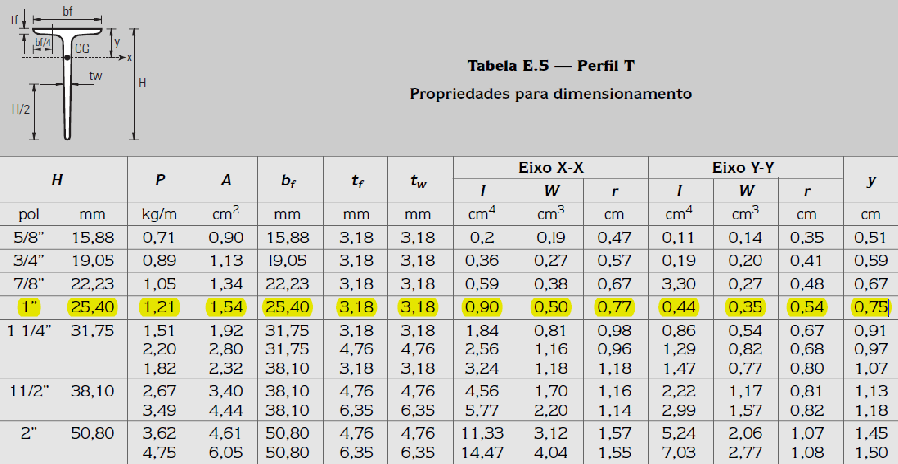
\includegraphics[width=0.8\textwidth]{figuras/perfil_t.png}
    \caption{Estrutura}
    \label{fig:awesome_image}
\end{figure}

\input{editaveis/energia_planejamento}
\chapter[Interações]{Interações Entre as Áreas}

O projeto Bike-x contará com a interação das engenharias de Software, Energia, Automotiva e Eletrônica. Esta seção visa identificar e exemplificar cada uma 
das interações. 

As engenharias de software e eletrônica vão se unir na área de coletar dados do sistema de forma geral e gerar informações relevantes a partir das mesmas. 
A área de engenharia eletrônica será responsável em fazer que os microcontroladores leiam dados de diversos sensores, tais como: oximetria e potenciômetro para 
definir a direção do guidão.  A engenharia de software irá processar esses dados e gerará informações para interagir com o usuário, informando os valores ou 
agindo no sistema.

As engenharias de energia e software irão interagir utilizando a eletrônica como intermediária. Haverá um sensor que medirá a quantidade de energia gerada 
pelo usuário e essa informação será tratada via software para que o usuário tenha acesso a essa informação de uma maneira agradável dentro do ambiente virtual.

As engenharias automotiva e de software também irão interagir utilizando a eletrônica como mediadora. Uma das interações com o sistema será que quando houver 
uma subida no ambiente virtual, o software irá gerar uma alteração no sistema. Quando isso houver, a bicicleta irá ser freada.

O sensor que mede a quantidade de energia produzida será responsável pela interação das engenharias de energia e eletrônica. Com esse sensor será possível 
mostrar ao usuário o quanto de energia ele conseguiu produzir. 

Durante uma subida no ambiente virtual, o sistema deverá frear a bicicleta para que o usuário sinta resistência ao pedalar e tenha a impressão de maior 
dificuldade de pedalar e que realmente pense que esteja em uma subida. Essa será a interação de engenharia eletrônica e automotiva.

Por fim, a interação das engenharias de energia e automotiva será feita pela adaptação do alternador no sistema para a geração de energia. Esse alternador 
será adaptado no rolo que usaremos para que o usuário possa pedalar sem se mover e com esse movimento a energia será gerada para alimentar o sistema.

\begin{figure}[h]
  \centering
    
  \def\firstcircle{(0:2.75cm)  circle (2.85cm)}
  \def\secondcircle{(90:2.75cm) circle (2.85cm)}
  \def\thirdcircle{(180:2.75cm) circle (2.85cm)}
  \def\fourdcircle{(270:2.75cm) circle (2.85cm)}

\tikzstyle{sensor}=[draw, fill=blue!20, text width=5em, 
    text centered, minimum height=2.5em,drop shadow]
\tikzstyle{wa} = [sensor, text width=10em, fill=red!20, 
    minimum height=6em, rounded corners, drop shadow]

  \begin{tikzpicture}[->,>=stealth',shorten >=1pt,auto,node distance=5cm,
  thick,scale=0.8]

    % The last trick is to cheat and use transparency
    \begin{scope}[shift={(3cm,3cm)}, fill opacity=0.5]
        \fill[red] \firstcircle;
        \fill[green] \secondcircle;
        \fill[blue] \thirdcircle;
        \fill[yellow] \fourdcircle;

        \draw \firstcircle node[right] (a) {$Software$}
        	[clockwise from=30,level distance=140,sibling angle=43]
			child { node[concept,text width=3cm,align=center] {Gerenciamento} }
			child {node[concept,text width=3cm,align=center] {Modelagem} }
			child { node[concept,text width=3cm,align=center] {Óculos de Realidade Virtual} }
        ;
        \draw \secondcircle node [above] (b) {$Eletrônica$}
        [clockwise from=90,level distance=170,sibling angle=30]
        	child { node[concept,text width=3cm,align=center] {Sensores} }
        ;
        \draw \thirdcircle node [left] (c) {$Energia$}
        [clockwise from=240,level distance=140,sibling angle=45]
        	child { node[concept,text width=3cm,align=center] {Armazenamento de Energia} }
        	child { node[concept,text width=3cm,align=center] {Conversão Electromecânica} }
        	child { node[concept,text width=3cm,align=center] {Eficiência Energética} }
        	child { node[concept,text width=3cm,align=center] {Distribuição} }
        ;
        \draw \fourdcircle node [below] (d) {$Automotiva$}
        [clockwise from=295,level distance=170,sibling angle=40]
        	child { node[concept,text width=3cm,align=center] {Ergonomia} }
        	child { node[concept,text width=3cm,align=center] {Analise Estrutural} }
        ;
    \end{scope}


\end{tikzpicture}
  \caption{Disponibilizações entre áreas}
  \label{intera}
\end{figure}


\chapter[Organização do Trabalho]{Organização do Trabalho}

Para a realização do projeto de forma eficiente e organizada, dividiu-se inicialmente o grupo em quatro subgrupos, cada um destes representando uma das 
engenharias (automotiva, eletrônica, energia e software), e cada subgrupo tendo um representante. No decorrer do projeto, de acordo com as demandas, os 
integrantes dos subgrupos deverão ser permutados. 

Haverá em média cinco reuniões semanais com duração de duas horas entre os integrantes do projeto, sendo três delas durante as aulas e duas extra classe.
O grupo decidiu utilizar uma abordagem ágil de gerenciamento de projeto, tendo em vista que a mesma funciona bem com times pequenos, concentrando ao máximo
o esforço do time em agregar valor ao produto proposto. Esse tipo de abordagem irá favorecer a integração do grupo de trabalho, objetivo principal da disciplina.

As decisões importantes a serem tomadas, como a definição do tema do projeto, as divisões e os principais resultados esperados, são feitas por 
todos os componentes do grupo durante os horários de reunião. Além das tomadas de decisões, as reuniões serão aproveitadas para cada subgrupo se reunir, 
trabalhar em sua determinada área, apresentar e discutir seus resultados obtidos para os demais subgrupos e, quando necessário, apresentar suas principais 
dificuldades e questionamentos para os professores da disciplina. Essas horas também serão úteis para que as tarefas em que é necessário mais de um subgrupo 
para sua realização sejam cumpridas através da reunião entre os mesmos para coletar as informações necessárias e discutir os melhores métodos e soluções para 
essas tarefas.

Foi estimada uma média de quatro horas semanais de trabalho além das seis horas de aula para cada componente do grupo, a fim de concluir as tarefas e metas 
propostas para cada um desses. Essas horas são utilizadas em sua maioria para pesquisas, testes, simulações e atualizações do relatório. 

Segundo \cite{XPxRUP2006}, metodologias ágeis também dividem o desenvolvimento do software em iterações, buscando redução de riscos ao projeto. Ao final de cada iteração, uma versão (release) funcional do produto, embora restrita em funcionalidades, é liberada ao cliente. As metodologias ágeis destacam aspectos humanos no desenvolvimento do projeto, promovendo interação na equipe de desenvolvimento e o relacionamento de cooperação com o cliente. Comunicação face-a-face é preferida à documentação compreensiva.

Com o objetivo de aperfeiçoar a integração entre os componentes dos grupos e para que cada um possa acompanhar o andamento do projeto são utilizadas algumas 
ferramentas e práticas ágeis, como \textit{software} de gerenciamento de projeto e \textit{daily meetings}. Assim, de modo que cada componente e/ou subgrupo 
possa acompanhar o que os outros estão fazendo no projeto está sendo utilizado: a ferramenta livre \href{http://lappis.unb.br/redm}{Redmine}, onde são apresentadas as tarefas, seus andamentos e o 
responsável por cada uma delas em um quadro \textit{kanban}; e os encontros diários, onde todos dizem o que foi feito, o que está sendo feito, as dificuldades
e o que será feito, possibilitando com que os principais problemas e dificuldades sejam detectados e solucionados por todos em conjunto. Para o agrupamento 
dos dados e pesquisas coletadas, além dos testes e resultados gerados e atualizações do relatório, é utilizada a ferramenta Google Docs.

Está sendo utilizada a ferramenta Git para realizar o controle de versão tanto dos códigos fonte gerados quanto dos documentos e apresentações, e como Source
Forge está sendo utilizado o GitHub. Sendo o Git uma ferramenta livre e o GitHub gratuito.

Com essa maneira de organizar o tempo, as tarefas e as equipes, espera-se que o andamento do projeto seja satisfatório, integrando as engenharias através do 
trabalho entre os subgrupos de maneira eficiente. Além disso, objetiva-se o melhor aproveitamento possível das horas disponíveis e determinadas para a realização 
do projeto por todos os componentes, de modo que a divisão de trabalho seja equilibrada ao longo do projeto, o que pode ser observado e analisado através das 
ferramentas utilizadas para o controle e divisão de tarefas.


\chapter[Organização das atividades]{Organização das atividades}
Para gerenciamento do projeto está sendo utilizada a ferramenta \href{http://lappis.unb.br/redm}{Redmine}, com esta ferramenta é possível fazer o gerenciamento do projeto no contexto ágil que é o que está sendo utilizado no Projeto.

Na figura dois abaixo observa-se o quadro de estórias (\textit{backlog}). O objetivo do quadro é pensar em todos os conjuntos de tarefas do projeto como um todo. Uma vez o quadro estando completo pode-se alocar as estórias em \textit{sprints}, que são ciclos de trabalho curtos com objetivos bem definidos. Na figura três observa-se um quadro de tarefas, que foi resultado de uma estória dividida em pequenas tarefas individuais.

\begin{figure}[h]
  \centering
  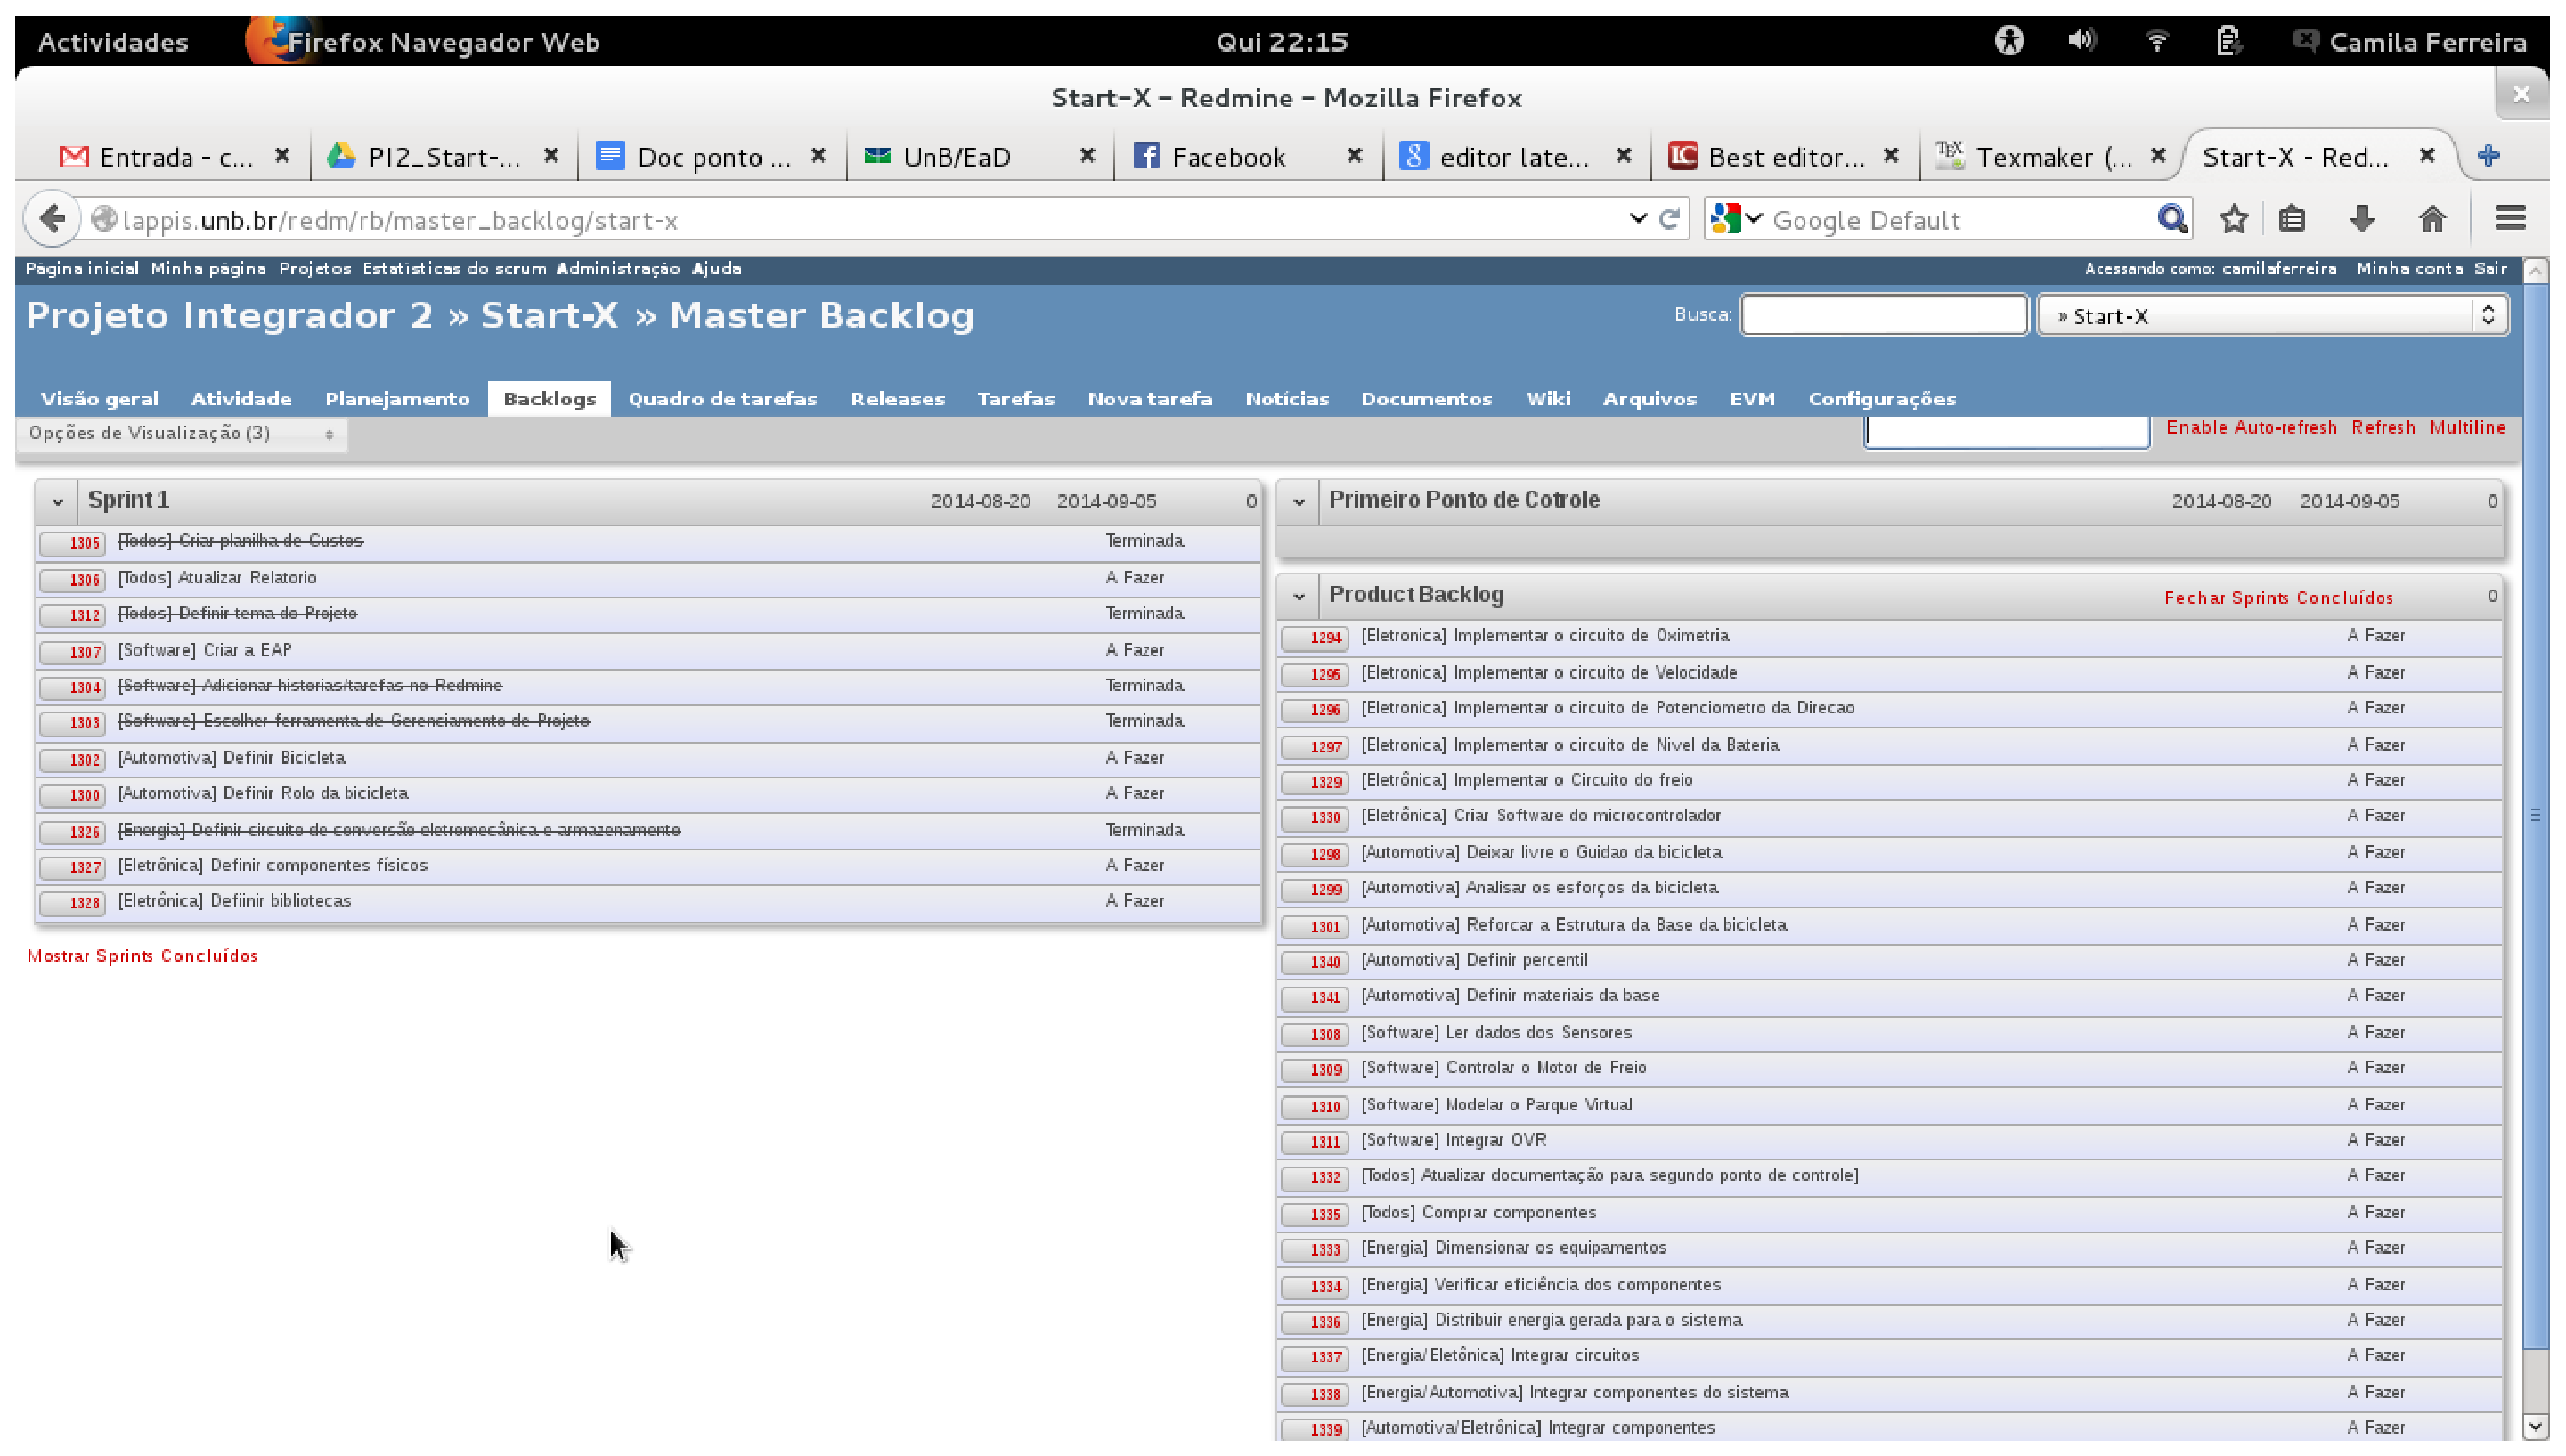
\includegraphics[width=0.7\textwidth]
      {figuras/backlogs.eps}
  \caption{Redmine e backlog do projeto}
  \label{redmine-backlog}
\end{figure}

\begin{figure}[h]
  \centering
  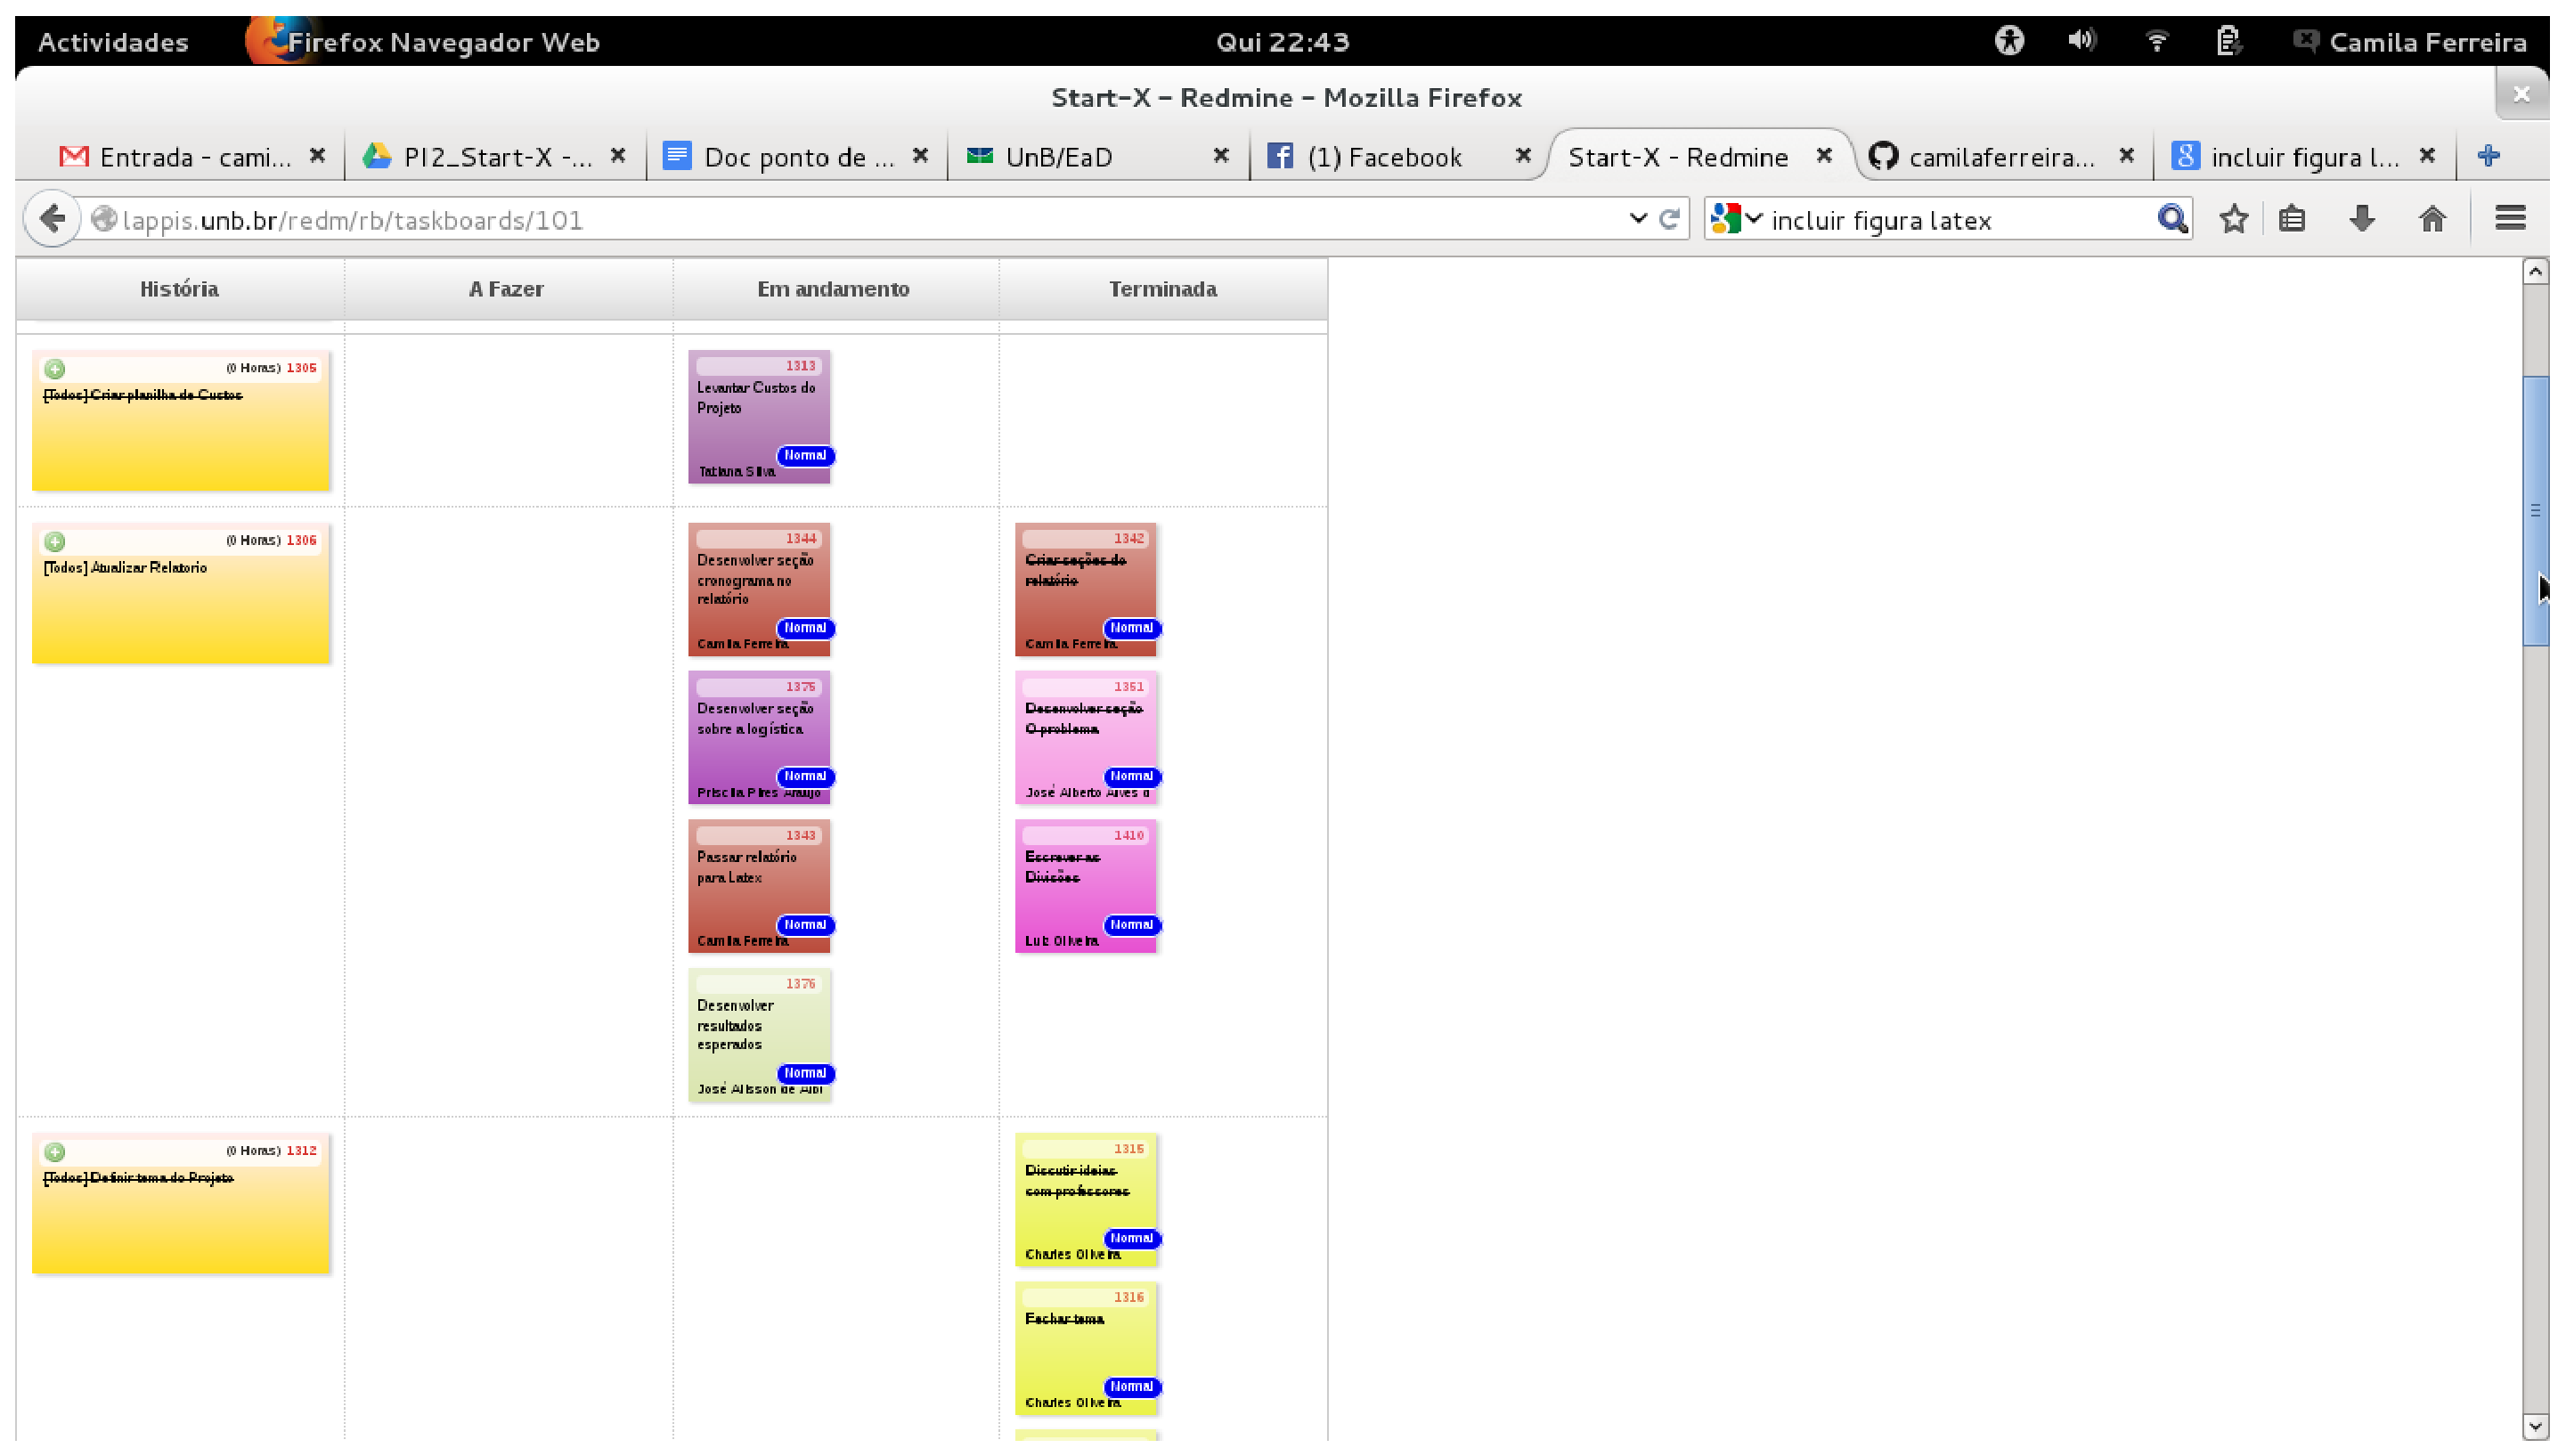
\includegraphics[width=0.7\textwidth]
      {figuras/quadrotarefas.eps}
  \caption{Quadro de tarefas}
  \label{quadro-de-tarefas}
\end{figure}
\newpage


\section{Cronograma}
Na figura quatro tem-se a Estrutura Analítica do Projeto - EAP, nela encontram-se os principais entregáveis do projeto. Com base nessa organização foi definido o seguinte cronograma para o projeto com três grandes pontos (datas a partir da Entrega 1 são aproximadas):
\begin{itemize}
  \item Entrega 1: 05/09/2014
    \begin{itemize}
      \item Viabilidade do projeto
    \end{itemize}
  \item Entrega 2: 31/10/2014
    \begin{itemize}
      \item Eng. Automotiva
        \begin{itemize}
          \item Ergonomia do produto
          \item Estrutura do produto
        \end{itemize}
      \item Eng. Eletrônica
        \begin{itemize}
          \item Montagem dos circuitos dos sensores
        \end{itemize}
      \item Eng. Energia
        \begin{itemize}
          \item Conversão eletromecânica
          \item Armazenamento de energia
          \item Eficiêcia energética
        \end{itemize}
      \item Eng. Software
        \begin{itemize}
          \item Modelagem do ambiente virtual
          \item Integração da modelagem
          \item Leitura dos dados dos sensores
        \end{itemize}
    \end{itemize}
  \item Entrega 3: 21/11/2014
    \begin{itemize}
      \item Energia/Software: Disponibilização dos dados de produção de energia
      \item Eletrônica/Software: Leitura dos sensores e informações no Oculus Rift
      \item Automotiva/Software: Acionamento dos freios em subidas virtuais
      \item Automotiva/Energia: Acoplamento da fonte motriz
      \item Eletrônica/Automotiva: Circuito que aciona os freios
      \item Eletrônica/Energia: Circuito controlador de energia produzida
    \end{itemize}
\end{itemize}
\begin{figure}[h]
  \centering
  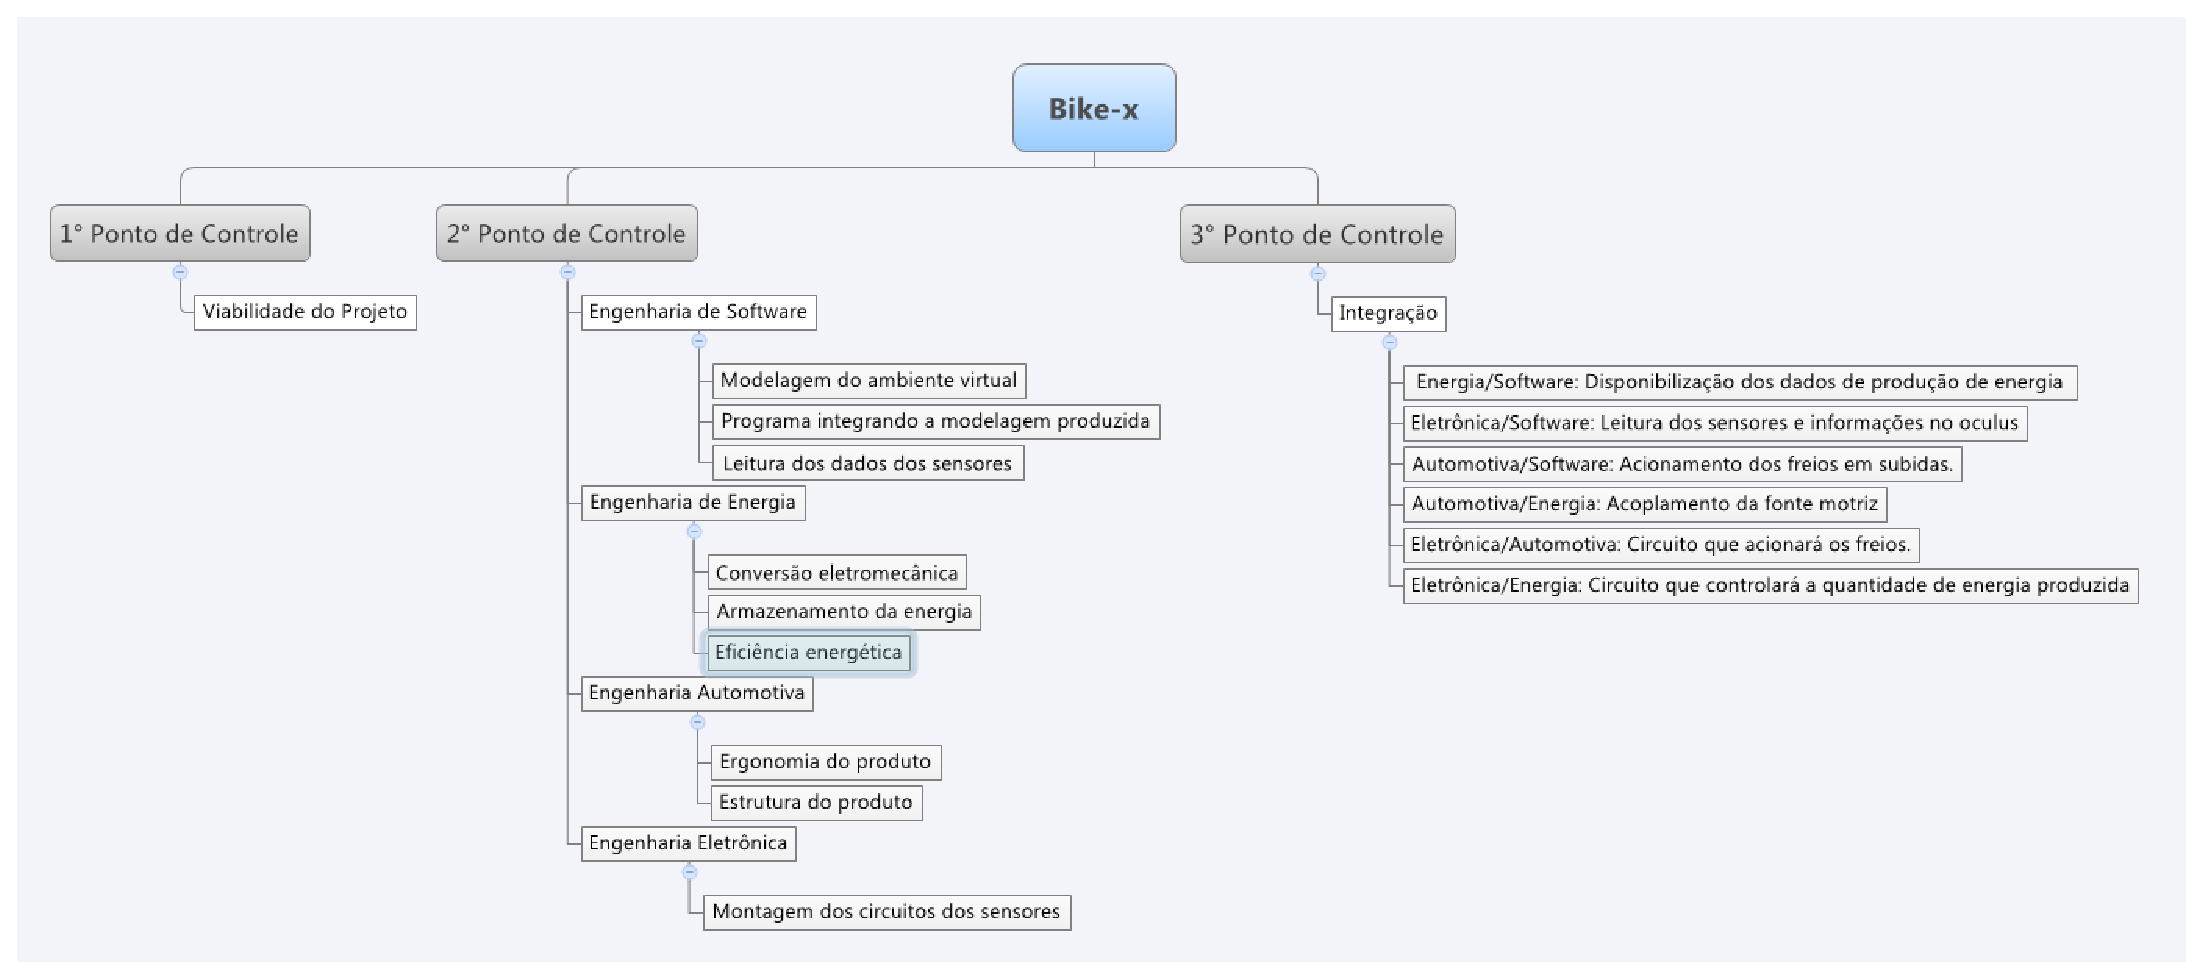
\includegraphics[width=1.2\textwidth, angle =90 ]
      {figuras/bike-x2.eps}
  \caption{EAP}
  \label{EAP}
\end{figure}




  

\chapter[Metas]{Metas}

Foram definidas 3 metas para o projeto:

\begin{itemize}
\item Definição do Projeto, esperamos definir o projeto bem como seu escopo.
\item Módulos funcionando separadamente, os módulos do produto devem estar funcionando separadamente
\item Produto concluído, a entrega do produto final com todos os módulos integrados e funcionando corretamente
\end{itemize}

\chapter[Financeiro]{Financeiro}
Foi feita estimativa dos custos do projeto em termos de recursos materiais. Os custos relativos à recursos humanos serão calculados e apresentados nos próximos relatórios.

\begin{table}[htbp]
\resizebox{\columnwidth}{!}{%
\begin{tabular}{|p{2.5cm}|p{4.5cm}|p{4.5cm}|p{2.5cm}|p{4.5cm}|}
\hline
\multicolumn{ 5}{|c|}{\textbf{Tabela de custos do projeto}} \\ \hline\hline
\multicolumn{1}{|p{2.5cm}|}{\textbf{Áreas}} & \multicolumn{1}{p{5cm}|}{\textbf{Descrição das etapas}} & \multicolumn{1}{p{4.5cm}|}{\textbf{Materiais}} & \multicolumn{1}{p{2.5cm}|}{\textbf{Quantidade}} & \textbf{Valores} \\ \hline \hline
\multicolumn{ 1}{|p{2.5cm}|}{\textbf{Engenharia Automotiva}} & \multicolumn{ 1}{p{5cm}|}{Compra da bicicleta, após definição do usário} & \multicolumn{ 1}{p{4.5cm}|}{Bicicleta} & \multicolumn{ 1}{p{4.5cm}|}{1 unidade} & \multicolumn{ 1}{p{4.5cm}|}{R\$140.00} \\ 
\multicolumn{ 1}{ |p{2.5cm}|}{} & \multicolumn{ 1}{p{5cm}|}{} & \multicolumn{ 1}{p{4.5cm}|}{} & \multicolumn{ 1}{p{4.5cm}|}{} & \multicolumn{ 1}{p{4.5cm}|}{} \\ \cline{ 2- 5}
\multicolumn{ 1}{ |p{2.5cm}|}{} & \multicolumn{ 1}{p{5cm}|}{Construção do suporte para bicicleta} & Barra de aço chato 1020 & \multicolumn{1}{p{4.5cm}|}{2 metros} & R\$24.00 \\ \cline{ 3- 5}
\multicolumn{ 1}{ |p{2.5cm}|}{} & \multicolumn{ 1}{p{5cm}|}{} & Barra de aço retang. 1020 & \multicolumn{1}{p{4.5cm}|}{2 metros} & R\$30.00 \\ \cline{ 3- 5}
\multicolumn{ 1}{ |p{2.5cm}|}{} & \multicolumn{ 1}{p{5cm}|}{} & Barra de aço circular 1020 & \multicolumn{1}{p{4.5cm}|}{1 metros} & R\$14.00 \\ \cline{ 3- 5}
\multicolumn{ 1}{ |p{2.5cm}|}{} & \multicolumn{ 1}{p{5cm}|}{} & Rolamento de alumínio (rolo) & \multicolumn{1}{p{4.5cm}|}{1 unidade} & R\$70.00 \\ \cline{ 2- 5}
\multicolumn{ 1}{ |p{2.5cm}|}{} & \multicolumn{ 1}{p{5cm}|}{Peças para encaixe da roda traseira} & Conjunto de parafusos/rosca/porcas & \multicolumn{1}{p{4.5cm}|}{x} & R\$40.00 \\ \cline{ 3- 5}
\multicolumn{ 1}{ |p{2.5cm}|}{} & \multicolumn{ 1}{p{5cm}|}{} & Manípulo de Aperto Amaciador & \multicolumn{1}{p{4.5cm}|}{2 unidades} & R\$10.00 \\ \cline{ 3- 5}
\multicolumn{ 1}{ |p{2.5cm}|}{} & \multicolumn{ 1}{p{5cm}|}{} & Borracha para fixação & \multicolumn{1}{p{4.5cm}|}{4 unidades} & R\$30.00 \\ \cline{ 2- 5}
\multicolumn{ 1}{ |p{2.5cm}|}{} & \multicolumn{1}{p{5cm}|}{Junção das barras para o suporte} & Soldagem & \multicolumn{1}{p{4.5cm}|}{x} & R\$60.00 \\ \hline
\textbf{} &  &  &  &  \\ \hline
 & \textbf{Subtotal} & \textbf{} & \textbf{} & \textbf{R\$418.00} \\ \hline
 % &  &  &  &  \\ \hline
 &  &  &  &  \\ \hline\hline
\multicolumn{ 1}{|p{2.5cm}|}{\textbf{Engenharia Eletrônica}} & \multicolumn{ 1}{p{5cm}|}{Leitura da velocidade do ciclista} & Circuito & \multicolumn{1}{p{4.5cm}|}{1 unidade} & R\$3.00 \\ \cline{ 3- 5}
\multicolumn{ 1}{ |p{2.5cm}|}{} & \multicolumn{ 1}{p{5cm}|}{} & Sensor de velocidade & \multicolumn{1}{p{4.5cm}|}{1 unidade} & R\$170.00 \\ \cline{ 2- 5}
\multicolumn{ 1}{ |p{2.5cm}|}{} & \multicolumn{ 1}{p{5cm}|}{Leitura dos batimentos cardíacos do ciclista} & Circuito & \multicolumn{1}{p{4.5cm}|}{1 unidade} & R\$3.00 \\ \cline{ 3- 5}
\multicolumn{ 1}{ |p{2.5cm}|}{} & \multicolumn{ 1}{p{5cm}|}{} & Sensor de oximetria & \multicolumn{1}{p{4.5cm}|}{1 unidade} & R\$10.00 \\ \cline{ 2- 5}
\multicolumn{ 1}{ |p{2.5cm}|}{} & \multicolumn{1}{p{5cm}|}{Leitura do nível da bateria} & Sensor de nível de bateria & \multicolumn{1}{p{4.5cm}|}{1 unidade} & R\$10.00 \\ \cline{ 2- 5}
\multicolumn{ 1}{ |p{2.5cm}|}{} & \multicolumn{1}{p{5cm}|}{Medir o giro do guidão} & Potenciômetro p/ guidão & \multicolumn{1}{p{4.5cm}|}{1 unidade} & R\$1.00 \\ \cline{ 2- 5}
\multicolumn{ 1}{ |p{2.5cm}|}{} & \multicolumn{1}{p{5cm}|}{Leitor dos sensores} & 1 micro msp 430 & \multicolumn{1}{p{4.5cm}|}{1 unidade} & R\$30.00 \\ \cline{ 2- 5}
\multicolumn{ 1}{ |p{2.5cm}|}{} & \multicolumn{1}{p{5cm}|}{Frenar a bicicleta} & Servo motor & \multicolumn{1}{p{4.5cm}|}{1 unidade} & R\$40.00 \\ \cline{ 2- 5}
\multicolumn{ 1}{ |p{2.5cm}|}{} & \multicolumn{1}{p{5cm}|}{Ventilação do ciclista} & Cooler & \multicolumn{1}{p{4.5cm}|}{2 unidade} & R\$100.00 \\ \hline
 &  &  &  &  \\ \hline
 & \textbf{Subtotal} &  &  & \textbf{R\$367.00} \\ \hline
 % &  &  &  &  \\ \hline
 &  &  &  &  \\ \hline \hline
\multicolumn{ 1}{|p{2.5cm}|}{\textbf{Engenharia de Energia}} & \multicolumn{1}{p{5cm}|}{Transforma energia mecânica em elétrica} & Alternador & \multicolumn{1}{p{4.5cm}|}{1 unidade} & R\$230.00 \\ \cline{ 2- 5}
\multicolumn{ 1}{ |p{2.5cm}|}{} & \multicolumn{1}{p{5cm}|}{Armazenamento de energia} & No break (bateria, tomadas e inversor) & \multicolumn{1}{p{4.5cm}|}{1 unidade} & R\$260.00 \\ \cline{ 2- 5}
\multicolumn{ 1}{ |p{2.5cm}|}{} & \multicolumn{1}{p{5cm}|}{Medição} & Multímetro & \multicolumn{1}{p{4.5cm}|}{2 metros} & R\$40.00 \\ \cline{ 2- 5}
\multicolumn{ 1}{ |p{2.5cm}|}{} & \multicolumn{ 1}{p{5cm}|}{Distribuição de energia} & Cabos (chicotes) & \multicolumn{1}{p{4.5cm}|}{1 unidade} & R\$18.00 \\ \cline{ 3- 5}
\multicolumn{ 1}{ |p{2.5cm}|}{} & \multicolumn{ 1}{p{5cm}|}{} & Cabos tipo jacaré & \multicolumn{1}{p{4.5cm}|}{4 unidade} & R\$16.00 \\ \hline
 &  &  &  &  \\ \hline
 & \textbf{Subtotal} &  &  & \textbf{R\$564.00} \\ \hline
 % &  &  &  &  \\ \hline
 &  &  &  &  \\ \hline \hline
\multicolumn{ 1}{|p{2.5cm}|}{\textbf{Engenharia de Software}} & \multicolumn{ 1}{p{5cm}|}{Óculos usado para simular ambiente virtual} & \multicolumn{ 1}{p{4.5cm}|}{Oculus Rift} & \multicolumn{ 1}{p{4.5cm}|}{1 undiade} & \multicolumn{ 1}{p{4.5cm}|}{R\$1,500.00} \\ 
\multicolumn{ 1}{ |p{2.5cm}|}{} & \multicolumn{ 1}{p{5cm}|}{} & \multicolumn{ 1}{p{4.5cm}|}{} & \multicolumn{ 1}{p{4.5cm}|}{} & \multicolumn{ 1}{p{4.5cm}|}{} \\ \hline
 &  &  &  &  \\ \hline
 & \textbf{Subtotal} &  &  & \textbf{R\$1,500.00} \\ \hline
 % &  &  &  &  \\ \hline
 &  &  &  &  \\ \hline \hline
 & \textbf{Total} &  &  & \textbf{R\$2,849.00} \\ \hline
\end{tabular}
}
\caption{Planilha de custos com equipamentos/materiais}
\label{fabela_fudida}
\end{table}

Considerando o valor médio ganho por um estagiário de Engenharia como 900,00 reais,
com 20 horas semanais temos que uma hora de um estagiário de engenharia equivale a
11,25 reais.

Consideramos 6 horas de trabalho por semana em 16 semanas dedicadas ao projeto Start-X.

\begin{table}[h]
\centering
\begin{tabular}{|l|c|l|}
\hline
Integrante       & \multicolumn{1}{l|}{Horas Trabalhadas} & Valor Total \\ \hline
Camila Ferreira  & 96                                     & R\$1,080     \\ \hline
Charles Daniel   & 96                                     & R\$1,080     \\ \hline
Gabriela Navarro & 96                                     & R\$1,080     \\ \hline
José ALberto     & 96                                     & R\$1,080     \\ \hline
José Alisson     & 96                                     & R\$1,080     \\ \hline
Júlio Cezar      & 96                                     & R\$1,080     \\ \hline
Lucas Kanashiro  & 96                                     & R\$1,080     \\ \hline
Luiz Fernando    & 96                                     & R\$1,080     \\ \hline
Macarcur Sousa   & 96                                     & R\$1,080     \\ \hline
Priscila Pires   & 96                                     & R\$1,080     \\ \hline
Tatiana Dias     & 96                                     & R\$1,080     \\ \hline
Thiago Ferreira  & 96                                     & R\$1,080     \\ \hline
\multicolumn{2}{|r|}{Total}                               & R\$12,960    \\ \hline
\end{tabular}
\caption{Planilha de custos com pessoal.}
\end{table}

Custo Total

\begin{table}[h]
\centering
\begin{tabular}{|l|l|}
\hline
Tipos de custo              & Valor       \\ \hline
Equipamentos/materiais      & R\$2,849.00 \\ \hline
Pessoal                     & R\$12,960   \\ \hline
\multicolumn{1}{|r|}{Total} & R\$15,809   \\ \hline
\end{tabular}
\caption{Custo total do projeto}
\end{table}


 
 

\part{Desenvolvimento}
Este capítulo descreve partes do sistema como um todo, abrangendo ferramentas de controle de estrutura, módulos de interface, hardwares envolvidos e afins. Serão apresentados os desenvolvimentos das partes de:

\begin{itemize}
	\item \nameref{software}
	\begin{itemize}
		\item Controle de infraestrutura
		\item Interface de controle
		\item Visualização de dados
	\end{itemize}
	\item \nameref{eletronica}
	\begin{itemize}
		\item Aquisição de dados
		\begin{itemize}
			\item Circuito do sistema
			\item Interface de aquisição e disponibilização dos dados (microcontrolador)
		\end{itemize}
	\end{itemize}
	\item \nameref{automotiva}
	\begin{itemize}
		\item Estrutura do produto e seus esforços
	\end{itemize}
	\item \nameref{energia}
	\begin{itemize}
		\item Acoplamento do alternador
		\item Cálculos de eficiência
	\end{itemize}
\end{itemize}


\chapter{Software}
\label{software}

\section{Puppet} % (fold)
\label{sec:puppet}

Para agilizar e evitar os problema com compatibilidades e erros de versões, foi utilizado a ferramenta \href{http://puppetlabs.com}{Puppet} para auxiliar com este processo administrativo de desenvolvimento do sistema.

\subsection{O que é o Puppet} % (fold)
\label{sub:o_que_o_puppet}

\gls{puppet} é um sistema de gerenciamento de configuração que permite que que seja definido o estado da infraestrutura de TI, em seguida, aplica automaticamente o estado correto. Para gerenciamento de alguns servidores ou maquinas, sejam elas físicas ou virtuais, o Puppet automatiza as tarefas administratidas do sistema que normalmente são feitas manualmente, liberando tempo e espaço mental dos administradores de sistemas para trabalhar nos projetos que proporcionam maior valor ao negócio.

\subsection{Integrando o puppet ao projeto} % (fold)
\label{sub:integrando_o_puppet_ao_projeto}

% subsection integrando_o_puppet_ao_projeto (end)

\section{Interface Python} % (fold)
\label{sec:interface_python}

A interface \gls{python} simplifica a comunicação com o microcontrolador, possibilitando o \textit{parse} entre o modulo principal (BikeX \ref{sec:sistema_bikex}) e o \gls{msp}.

A interface faz de uso da biblioteca \href{http://pyserial.sourceforge.net/pyserial.html}{Pyserial} para manter a comunicação com o microcontrolador. Devido as inúmeras possibilidades de conflitos existentes de caracteres e velocidade de comunicação existentes na comunicação \gls{rs232}, os desenvolvedores da \textit{Pyserial} construíram a classe \textit{serial.tools.miniterm} na qual simula um terminal de comunicação como exemplo de uso da biblioteca. O grupo construiu então uma classe que herda da \textit{serial.tools.miniterm}, simplificando assim a comunicação e incrementando a estabilidade de comunicação. Esta ação gera a dependência de que a versão da \textit{Pyserial} necessita ser 2.7 ou superior.

\subsection{Visão do BikeX} % (fold)
\label{sub:vis_o_do_bikex}

Do ponto de vista do BikeX a aplicação Python estará rodando sempre em \textit{background} esperando um sinal para a realização de alguma tarefa. A depender do sinal recebido, será realizado uma leitura do estado dos sensores ou o envio do valor de posicionamento do freio.

% Por ser um programa assíncrono, a aplicação passará grande parte do tempo ociosa.
A tomada de uso de sinais para acordar o processo possibilita que o mesmo se mantenha em descanso durante todo o período em que não há requisição de dados. Como resultado do ponto de vista da arquitetura que suportado software, não há uma sobrecarga de processamento, evitando o \textit{overhead} de requisições desnecessárias e possibilitando assim que o processamento possa ficar focado onde realmente há uma grande demanda de CPU e GPU, que é a interface gráfica da aplicação.

No trecho de código a seguir (\ref{trecho_main_py}) é possível observar a rotina principal da aplicação \textit{Python} populando o objeto do MSP430 com alguns dispositivos e definindo os métodos a serem chamados na ocorrência dos sinais já pré-definidos. Em seguida o programa entra no já referido \textit{loop}, permanecendo nele ate receber um sinal que requisite o termino do processo.

\begin{lstlisting}[language=Python,caption={Trecho da rotina principal do script Python},label=trecho_main_py]
def main():
    pid_bikex = sys.argv[1:2]
    msp430.curb = sensor.Break(msp430.serial,0)
    msp430.velocity = sensor.Velocity(msp430.serial,0)
    msp430.passives = sensor.Passives(msp430.serial,0)


    signal(SIG1, write_file)
    signal(SIG3, read_file)
    signal(SIGINT, safe_quit)
    signal(SIGQUIT, safe_quit)
    signal(SIGABRT, safe_quit)
    while True:
        sleep(0.01)

\end{lstlisting}


\subsection{Visão do MSP430} % (fold)
\label{sub:vis_o_do_msp430}

Do ponto de vista do MSP430 a aplicação Python estará sempre em comunicação ativa com o MSP430, já que a porta serial será aberta assim que o sistema for iniciado e só fechará quando programa vier a fechar.

Como apresentado no código \ref{trecho_main_py}, a aplicação Python estará sempre a espera de um sinal para entrar em contato com o MSP430. Para que ocorra a interação, é enviado um comando especifico ao MSP430 sobre qual dispositivo desejamos ter informação. No código \ref{trecho_device_py} podemos observar a declaração de algumas classes de dispositivos passivos na estrutura física do projeto, como o freio. Todos os dispositivos herdam de uma classe primaria que tem declarada uma sequencia básica de leitura-escrita de comandos no MSP430.


\begin{lstlisting}[language=Python,caption={Declaração de classes fundamentais no script Python},label=trecho_device_py]
class Passive(Device):
    """docstring for Active"""
    def __init__(self, terminal):
        super(Passive, self).__init__(terminal)
        self.data = self.serial.readline()
        self.data = self.data.split('\n')[0]

    def read_data(self, command):
        """ Send some data to device """
        self.serial.write(str(command))
        self.data = self.serial.readline()
        self.data = self.data.split('\n')[0]
        return self.data

    def write_data(self, command, data):
        return None

class Velocity(Passive):
    """docstring for Velocity"""
    def __init__(self,terminal, arg=VELOCITY_MSP):
        super(Velocity, self).__init__(terminal)
        self.arg = arg
        
    def read_data(self):
        return super(Velocity, self).read_data(self.arg)

class Passives(Passive):
    """docstring for Passives"""
    def __init__(self,terminal, arg=ALL_VALUES):
        super(Passives, self).__init__(terminal)
        self.arg = arg
        
    def read_data(self):
        return super(Passives, self).read_data(self.arg)
\end{lstlisting}

Definido uma interface padrão de leitura-escrita nos dispositivos, é então instanciado no objeto \textbf{MSP} a os dispositivos desejados para que a rotina principal possa interagir com os dispositivos. Para uma mair comodidade e melhor visualização da escrita do código, foram definidos os métodos \textit{\_\_getitem\_\_} e \textit{\_\_setitem\_\_} da classe \textbf{MSP}, conforme apresentado a seguir:

\begin{lstlisting}[language=Python,caption={Declaração dos métodos de leitura e escrita de item},label=trecho_item_py]
    def __getitem__(self,key):
        """ Return the value of a item """
        try:
            return getattr(self,key).read_data()
        except Exception, e:
            raise e

    def __setitem__(self,key,item):
        """ Set a value of a item """
        getattr(self,key).write_data(str(item))
\end{lstlisting}

As rotinas implementadas no trecho do código \ref{trecho_item_py} permitem a leitura e o envio de algum valor, respectivamente, de um possível atributo \textit{foo} - meramente ilustrativo de exemplo - da seguinte forma:

\begin{lstlisting}[frame=none,numbers=none]  % Start your code-block

>>> msp430.foo = sensor.Passives(msp430.serial,0)
>>> print msp430['foo']
>>> 33
>>> """Sending some value"""
>>> msp430['foo'] = 30
\end{lstlisting}

	Obviamente que, como visto no código \ref{trecho_device_py}, o método de escrita de objetos passivos se resume a retornar um objeto nulo, não interagindo assim com o MSP430. Porém, esta solução permite que, se houvesse o interesse em fazer de uso de algum dispositivo no MSP430 que pudesse assumir estados e retornar valores, a interação com ele seria a mais transparente possível. Um possível exemplo seria uma segunda porta de comunicação, seja ela UART ou algum outro protocolo de comunicação como $CAN$ ou $I^2C$. Da mesma forma que poderíamos enviar uma \textit{string} pela UART para ser equalizada na outra porta, poderíamos receber uma mensagem nova pela mesma.

% Os códigos na integra podem ser observados nas sessões \ref{main_py}, \ref{device_py} e \ref{msp430_py}  nos anexos.

\section{Sistema BikeX}
\label{sec:sistema_bikex}

%Software Bikex: modelagem (uml), linguagem, signals, arquitetura
\subsection{Módulos}
Esta seção visa descrever como os diversos módulos do sistema irão se comportar separadamente e como vão interagir entre si. O sistema será composto pelos Unity, Bikex, Device. A figura \ref{diagrama-classes} exemplifica como os módulos interagem entre si.

O módulo Unity será responsável com as interações entre o usuário e o sistema. A primeira responsabilidade é retornar para o sistema a altitude atual do usuário. Essa informação será usada para definir se é necessário o acionamento da frenagem para simular uma inclinação no ambiente virtual. Outra responsabilidade será definir a posição e rotação atual do usuário no sistema. Essas informações irão ser disponibilizadas com a interação de outros módulos. Algumas informaçòes serão disponibilizadas pelo sistema para o usuário. Informações como: velocidade, distância e a velocidade máxima atingida pelo usuário. Por fim, esse módulo irá fazer a renderização do frame para o usuário. Essa renderização irá considerar todas as interações com o sistema e as informações geradas com essa interação.

\begin{figure}[h]
  \centering
	%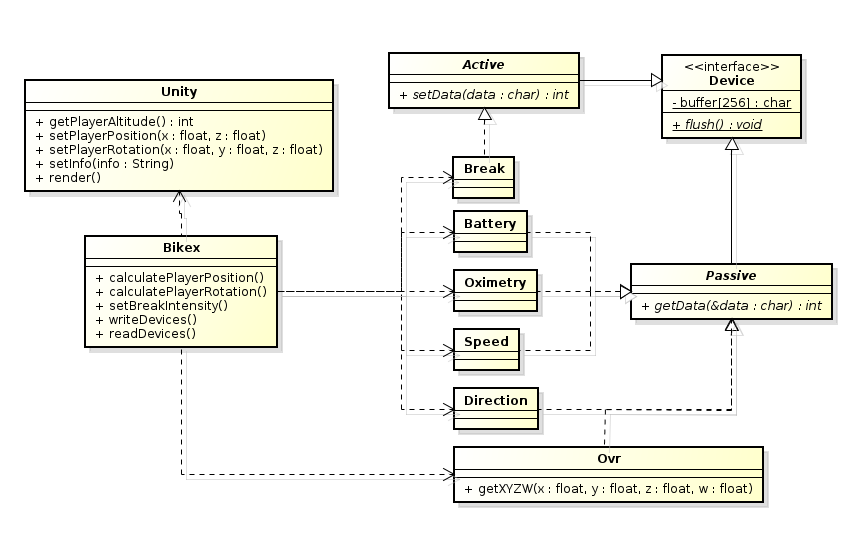
\includegraphics[scale=0.5]{figuras/diagrama_de_classe}
  \caption{Diagrama de classes}
  \label{diagrama-classes}
\end{figure}

No sistema terá um módulo que será composto por várias classes. Esse módulo, que é o responsável em fazer a interação com os dispositivos externos, se chama Device. Primeiramente, a classe principal será uma interface chamada Device. Duas classes irão relacionar com essa interface diretamente, a Active e a Passive. A classe Active representará os dispositivos que irão influenciar ativamente e fisicamente no sistema. Essa classe irá ser responsável por informar os dados para essa influência no sistema. Um dispositivo que exemplificar é a frenagem do sistema. A classe Passive são dispositivos que fornecem informações para o sistema. Os dispositivos de velocidade, direção e OVR são exemplos desse tipo de Device. A classe Passive irá ser responsável de coletar informações desses dispositivos e fornecer para o sistema realizar os procedimentos necessários. O dispositivo OVR é o Oculus em si e será responsável em fornecer a posição da cabeça do usuário.

O módulo Bikex é o módulo central do sistema e fará a interface com o módulo Unity e os outros módulos. Esse módulo é responsável por receber as informações dos dispositivos do tipo Passive e fazendo as transformações necessárias para enviar para o módulo Unity. O primeiro procedimento que esse módulo realiza é o cálculo da posição do usuário e tem como entrada a velocidade e a direção atuais do usuário. Outro procedimento será o cálculo da rotação do usuário. Isso será feito a partir de dados fornecidos pelo dispositivo Oculus. Essa rotação definirá a direção que o usuário está olhando. Definimos a separação desses dois procedimentos para que a rotação da cabeça do usuário não interfira na rotação da bicicleta. O outro procedimento é definir a intensidade de frenagem de acordo com a altitude coletada do módulo Unity. A partir dessa intensidade, o Bikex aciona o dispositivo de freio com a mesma.



%Unity: scripts, modelagem, assets etc
\subsection{Unity}

%Python: versao do python, modulos puppet, modulos para comunicacao UART
\subsection{Python}

%Falar aqui sobre o software do bikex, a integracao do python/msp430/unity
\subsection{Integração Sensores e Sistema}

\section{Funcionamento do Oculus Rift}
O Oculus Rift é basicamente uma lente com uma tela de alta resolução juntamente com sensores e giroscópios trabalhando em conjunto. A sensação de imersão vem com a baixa taxa de resposta entre o movimento do usuário e a imagem gerada na tela, fazendo com que a experiência se torne algo prazeroso e comfortável.

\subsection{Esquema de coordenadas}
Para manter a rastreabilidade dos movimentos da cabeça do usuário, o Oculus Rift trabalha com um sistema de coordenadas parecido com o da regra da mão direita. A figura abaixo ilustra como os eixos e sentidos são levados em consideração para o Rift.
\begin{itemize}
  \item Y é positivo para cima
  \item X é positivo para direita
  \item Z é positivo para traz
\end{itemize}
A rotação é mantida como uma unidade quaternária, mas também pode ser reportada na forma \textit{yaw-pitch-roll}. Os termos vêm do inglês e significam, respectivamente, giro, arremesso e rolo. Cada um dos eixos geram valores que significam as rotações (positivas ou negativas) de acordo com o movimento da cabeça do usuário:
\begin{itemize}
  \item \textit{Pitch} é a rotação entorno do eixo X, positivo quando arremessado para cima
  \item \textit{Yaw} é a rotação entorno do eixo Y , positivo quando virado para esquerda
  \item \textit{Roll} é a rotação entorno do eixo Z, positivo quando se encosta a cabeça no ombro esquerdo
\end{itemize}

\begin{figure}[h]
  \centering
  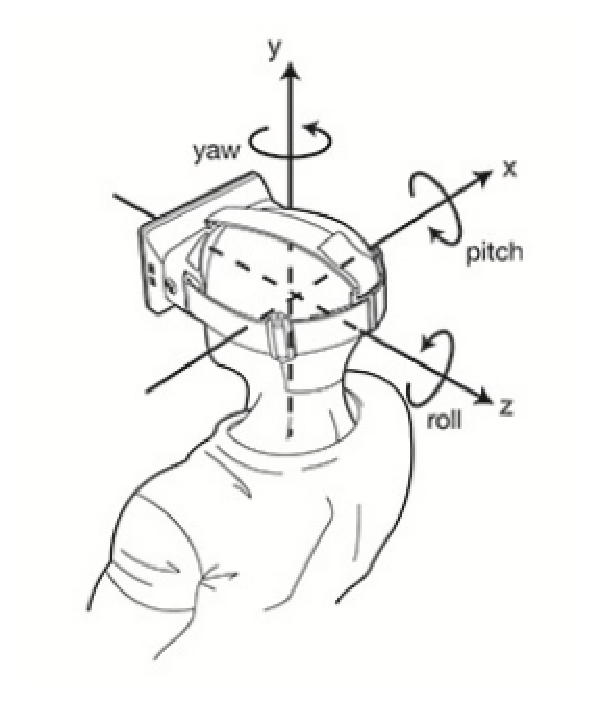
\includegraphics[width=0.5\textwidth]
      {figuras/esquema_coordenadas_rift.eps}
  \caption{Esquema de coordenadas do Oculus Rift}
  \label{coordenadas-rift}
\end{figure}

\subsection{Distorção}
O Oculus Rift requer que a cena seja renderizada em uma tela dividida com metade da tela usada para cada olho. Ao usar o aparelho, o olho esquerdo enxerga a metade esquerda da tela e o olho direito a metade direita. Por mais que varie de pessoa para pessoa, a distância das pupilas de um ser humano estão, aproximadamente, 65 mm longes uma da outra. Essa distância é conhecida como \textit{interpupillary distance}(IPD), ou distância interpupilar. Essa distância deve ser levada em consideração ao se escolher a distância entre as câmeras que captam as cenas na aplicação. Observe que o IPD se refere à translação da câmera, e não à rotação, e é essa translação que causa o efeito esteroscópico*. Isso significa que a sua aplicação precisará de renderizar a cena inteira duas vezes, uma para a metade esquerda e outra para a metade direita. 

As lentes do Oculus Rift ampliam a imagem para proporcionar grande \textit{field of view} (FOV), ou campo de visão, (quase total) que melhora muito a imersão virtual, basicamente não se vê outra coisa além do \"ambiente\" gerado pelas telas. Entretanto, as lentes distorcem a imagem final signicativamente até o ponto do usuário enxergar a distorção de almofada (distorcida \"para dentro\"). Para reverter a distorção da lente, deve haver a aplicação de um pós-processamento nas imagens renderizadas a fim de distorcê-las \"para fora\" (distorção de barril), figura abaixo. Sendo assim, os desenvolvedores implementaram uma API para aplicar distorção na imagem com o objetivo de ser cancelada pela lente do Rift. Finalmente, a API também trata o efeito chamado \"effeito arco-íris\" causado pelas bordas da lente. Mesmo que os parâmetros de distorção dependam das características da lente e da posição relativa dos olhos em relação a lente, a API cuida de todos os aspectos de geração da distorção, gerando uma imagem final no Oculus sem distorção alguma.

\begin{figure}[h]
  \centering
  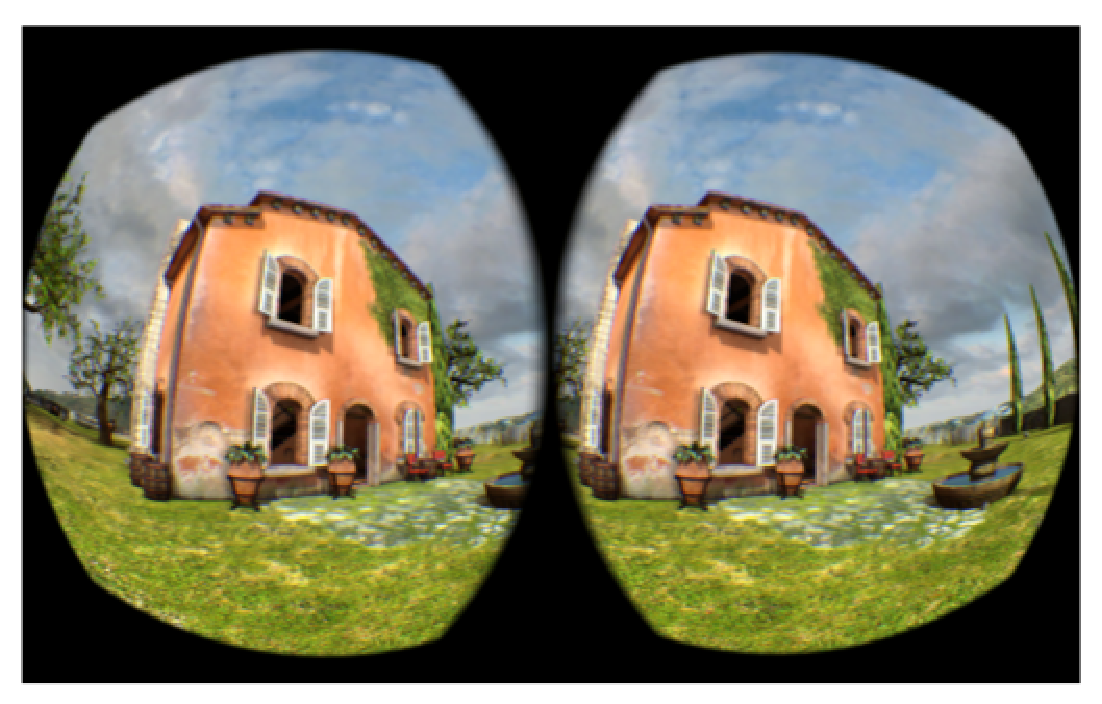
\includegraphics[width=0.7\textwidth]
      {figuras/distorcao_barril.eps}
  \caption{Imagem com distorção de barril}
  \label{coordenadas-rift}
\end{figure}

A projeção dos eixos das câmeras deve ser paralela uma com a outra como na figura abaixo. As vistas esquerda e direita são independentes uma da outra, isso significa que a configuração das câmeras da aplicação é basicamente a mesma ao se utilizar uma câmera única, a diferença é a distância entre os dois eixos ao se criar uma cena para o Rift.

\begin{figure}[h]
  \centering
  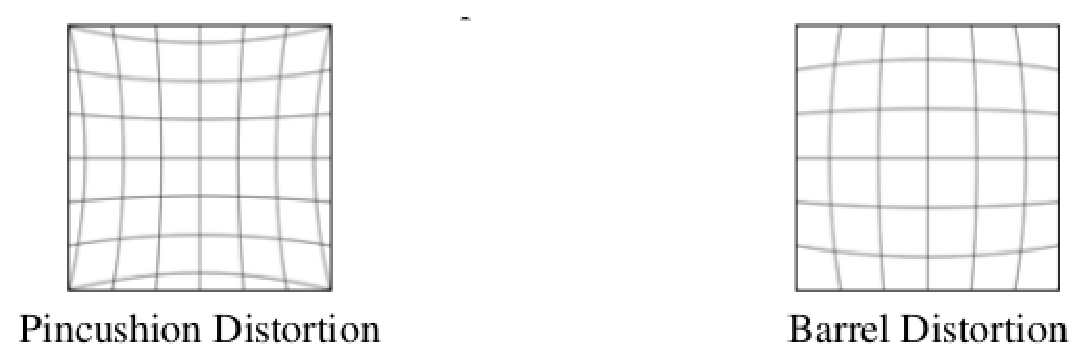
\includegraphics[width=0.7\textwidth]
      {figuras/distorcao_rift.eps}
  \caption{Distorção de lentes e imagens do Rift}
  \label{coordenadas-rift}
\end{figure}

\section{Ambiente virtual}

O Unity 3D é uma das ferramentas mais usadas para criar jogos para as mais diversas 
plataformas, e diferente do que muitos acreditam o software pode ser muito simples 
de usar quando se conhece o seu funcionamento básico. É possível criar jogos e 
aplicações interativas no Unity para Web, Desktop, iOS, Android e até mesmo 
consoles como PS3, XBOX 360 e Wii.

Para iniciar a modelagem do Parque Virtual foi escolhido um mapa em escala de 
cinza para que sirva de base para o ambiente virtual. O mapa foi adaptado para 
que fosse reconhecido pelo Unity.

\begin{figure}[htpb]
 \begin{center}
    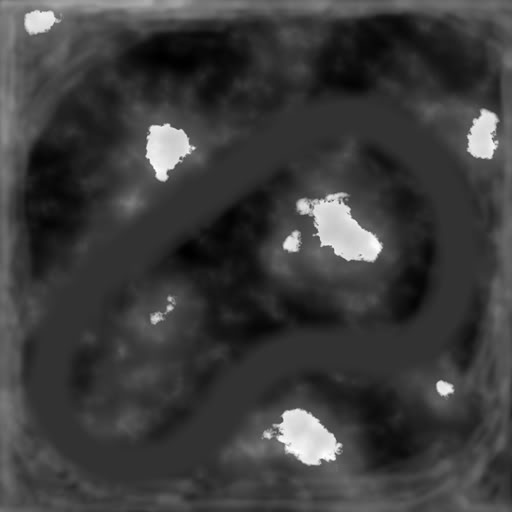
\includegraphics[width=.40\textwidth]{figuras/mapa.jpg}
 \end{center}
  \caption{Mapa do ambiente virtual em escala de cinza}
  \label{fig:core_concurrent}
\end{figure}

O mapa foi importado para o Unity e foi colocada nele uma base de grama para que
os outros componentes sejam colocadas por cima desta base.

Foi feita uma adequação do terreno formado pelo mapa de cores para que fosse criada
a ciclovia e na parte mais baixa do mapa foi adicionado água para termos pequenos 
lagos.

Os elementos que estão sendo adicionados no conforme idéias e necessidades encontradas
pela equipe, primeiramente inserimos algumas árvores e vegetações para dar uma visão
de parque ao mapa, inserimos também uma ponte para que o usuário possa passar por um 
ponto de água, está sendo elaborado um túnel para que o usuário possa passar no 
ambiente.  



\section{Circuitos e sensores}
colocar aqui os layouts dos circuitos e sensores usados (velocidade, motor e direcao (se der tempo, poe tbm o de oximetria e o da bateria))
\section{MSP430} % (fold)
\label{sec:msp430}

É um microcontrolador RISC de 16 bits criado pela Texas Instrumets para aplicações de baixo consumo de energia.

% Colocar aqui sobre o que é o MSP430, sua função no projeto como foi utilizado


\subsection{MSPGCC} % (fold)
\label{sub:mspgcc}

%This is a port of the GNU C Compiler (GCC) and GNU Binutils (as, ld) for the embedded processor MSP430. Tools for debugging and download are provided (GDB, JTAG and BSL)
% subsection mspgcc (end)
\chapter[Automotiva]{Automotiva}
\label{automotiva}


\section{Base da bicicleta}
Colocar aqui os calculos dos esforcos da bicicleta, os calculos pra fazer a base, se puder colocar a foto da modelagem (no catia?) da base tbm ia ser bom
\chapter{Energia}
\label{energia}


\section{Acoplamento do alternador}
Mostrar onde o alternador vai ser acoplado na base da bicicleta, como a roda vai girar o alternador, qual a forca a ser aplicada na pedalada pra mover o alternador...Colocar fotos e modelagens (do catia?)
(A energia gerada sera apresentada aqui tbm ? )



% subsection tac_metro (end)
\begin{figure}[h]
	\centering
	\begin{circuitikz}[american,scale=0.8,
		start chain=going right,
		diamond/.style={
			on chain,join,draw,
			minimum height=3cm,
			text centered,
			minimum width=2cm,
		},
		every join/.style={ultra thick}]

	\draw
	(-26,0) node[transformer core] (T) {}
	(T.A1) node[anchor=east] {} %A1
	(T.A2) node[anchor=east] {} %A2
	(T.B1) node[anchor=west] {} %B1
	(T.B2) node[anchor=west] {} %B2
	;

	\draw (-23,-1.5)
		to[short,n=d1]++(0,0) to [D*,*-*] ++(45 :2)
		to[short,n=d2]++(0,0) to [D*,*-*] ++(-45 :2);
	\draw (-23,-1.5)
		to[short,n=d3]++(0,0) to [D*,*-*] ++(-45 :2)
		to[short,n=d4]++(0,0) to [D*,*-*] ++(45:2) to[short,n=_d4]++(0:0)
		;

	\draw
	(T.A2) to  [sinusoidal current source,l^=$\frac{14V}{35A}$,n=cap] ++(0,2.5) to  (T.A1)
	(T.B1) |- (d2)
	(T.B2) |- (d4)
	(_d4) to [short,n=center] ++(5,0)
	(center) to [R,l_=$R_1$,*-] ++(0,3) to [zD*,l_=$Z_1$]++(0,2) to [fuse,l_=$F_1$,-o]++(4,0)
	(center) to [R,l_=$R_2$,mirror]++(0,-3) to [fuse,l_=$F_2$]++(0,-2) to [D*,l_=$D_1$,n=dio]++(4,0) 
	(center) to [fuse,l_=$F_3$]++(6,0) to [short]++(1,0) to [cspst,l^=$Ch_1$]++(0,-3) to [short,n=end]++(0,-2) to [battery,l_=$\frac{12V}{7Ah}$,*-]++(-3,0) to (dio)
	(end) to [cspst,l^=$Ch_2$]++(0,-4) to [short,n=baixo]++(0,-0.5) to [lamp]++(0,-1)
	(d3) to[short]++(-1,0) |- (baixo)
	;

	\end{circuitikz}
	\caption{Circuito do Alternador}
	\label{circ}
\end{figure}
\section{Eficiência energética}

\subsection{Levantamento das Cargas}
\label{levantamento-cargas}

Nesta seção cuidar-se-á em informar as características nominais das cargas que serão alimentadas pela energia elétrica gerada a partir da conversão da energia mecânica existente devido ao torque exercido no eixo da bicicleta pelo usuário do projeto. Assim, apresenta-se a Tabela xxx, a qual indica aquelas características daquelas cargas.
Sensores, celular (tensão nominal, fator de potência, potência requerida, corrente, potência aparente, faixa de tensão etc.).

\subsection{Fonte Geradora}
\label{fonte-geradora}

\subsubsection{Princípio de Funcionamento do Gerador Síncrono}
\label{gerador-sincrono}


Geradores síncronos são bastante utilizados em centrais elétricas, independente do seu tipo. Grande parcela da energia elétrica disponível mundialmente é gerada por esse tipo de geradores, que convertem energia mecânica em energia elétrica. Além da geração de energia elétrica para ser distribuída na rede elétrica, os geradores síncronos são usados na geração de energia de pequeno porte e autônoma, não conectada a rede elétrica, como é o caso do presente projeto. 
Uma máquina síncrona é constituída por enrolamentos de armadura alojados na parte estacionária, denominada estator. Esses enrolamentos são conhecidos como enrolamentos do estator. Além deles, há um segundo enrolamento denominado enrolamento de campo, no qual gera corrente contínua e é utilizado para produzir o principal fluxo de operação do gerador. Em um gerador síncrono, o enrolamento de campo encontra-se no rotor, de modo que a corrente em que a corrente deve ser fornecida através do contato rotativo mecânico.  Segundo Fitzgerald, é vantajoso em um gerador síncrono que o enrolamento de campo, único e de baixa potência, localize-se no rotor e o enrolamento de armadura, de potência elevada e geralmente polifásico, encontre-se no estator.
O princípio de funcionamento de um gerador síncrono assemelha-se ao de uma máquina de corrente contínua no que diz respeito à tensão induzida no condutor, gerada pelo movimento rotativo entre um condutor e um campo magnético. Em um gerador síncrono, os condutores são fixos na armadura e o campo magnético é forçado pela máquina primária a se mover. A máquina primária é acoplada ao rotor do gerador, onde se encontram os polos, submetendo-os a uma força que os fazem girar. Como consequência do movimento entre o condutor e o campo, surge a tensão nos terminais do gerador síncrono, na qual faz com que uma corrente circule pelo gerador e pela carga que será ligada no gerador. Com a tensão e a corrente induzida pelo movimento, a potência mecânica transferida pela máquina primária é então convertida em energia elétrica, levando em consideração as perdas existentes nesse fenômeno. O enrolamento de campo é alimentado por uma fonte de corrente contínua por meio de anéis deslizantes. A tensão gerada pelo gerador síncrono trata-se de uma tensão alternada senoidal, que pode ser monofásica ou trifásica.
Com o objetivo de aumentar a potência convertida, em um gerador síncrono não há apenas um condutor sendo movimentado no campo magnético, mas condutores ligados em série. Assim, a potência do gerador e o aproveitamento dos materiais são maiores. 

\subsubsection{Partes Construtivas do Gerador Síncrono}
\label{construtivas-gerador-sincrono}

O alternador é composto das seguintes partes: rotor, estator, carcaça, escova e anéis, ponte retificadora, ventilador, polias e parafusos. As principais partes construtivas de um alternador serão tratadas posteriormente no presente relatório.
Abaixo, na figura \ref{partes-alternador}, são mostradas essas partes que compõem um alternador de automóvel.


\begin{figure}[h]
	\centering
	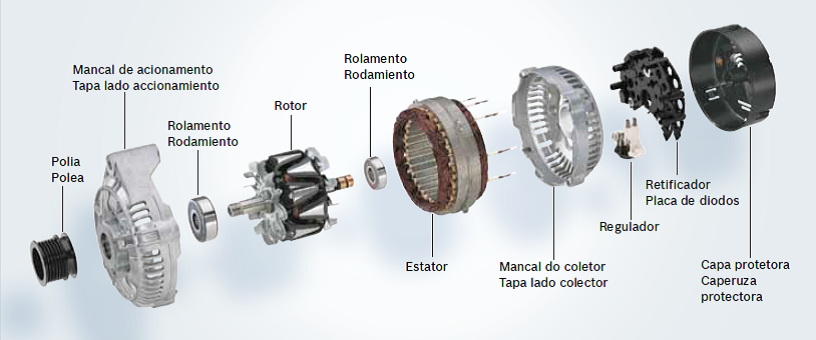
\includegraphics[scale= 0.8]		{figuras/partes_alternador.png}
	\caption{Partes que compõem um alternador}
	\label{partes-alternador}
\end{figure}

\begin{description}

\item [Rotor]
O rotor é trata-se da parte móvel no centro do alternador, constituído por um eixo de aço com uma bobina enrolada em seu interior, na qual a quantidade de fios de cobre da bobina varia de acordo com a capacidade e especificações de cada alternador. O rotor tem como principal função formar um campo magnético que tem como resultado a produção de corrente elétrica, onde os seus polos são alimentados com corrente contínua e geram o campo principal que induz tensão na armadura. A alimentação do enrolamento de excitação no alternador utilizado é feito através de anéis e escovas. 
Abaixo, na figura \ref{rotor-alternador}, pode ser visto o rotor do alternador utilizado no presente trabalho, representado pelo número 1.

\begin{figure}[h]
	\centering
	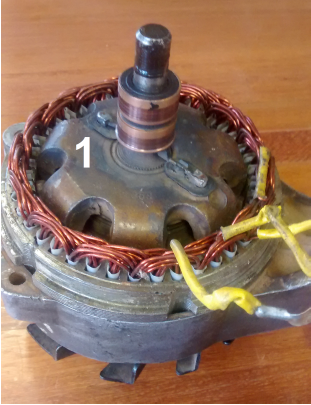
\includegraphics[scale=0.8] {figuras/rotor_alternador.png}
	\caption{Rotor do alternador}
	\label{rotor-alternador}
\end{figure}

\item [Estator]

O estator é formado por um conjunto de bobinas isoladas entre si e fixadas em um conjunto de laminas de aço. Essas lâminas têm características magnéticas de alta permeabilidade, proporcionando um caminho com pequena relutância para o fluxo, o que diminui o fluxo disperso e concentra o campo no entreferro. O uso de lâminas na construção do estator proporciona a diminuição das perdas provocadas por correntes parasitas em relação ao emprego de uma estrutura maciça. Essas lâminas também são tratas termicamente para diminuir o valor das perdas geradas por correntes induzidas.
Essa parte fundamental de um gerador síncrono tem como principal função a criação da corrente elétrica. Entretanto, para a geração de energia as boninas do estator requerem a produção de um campo magnético pelo rotor. A figura \ref{estator-alternador} apresenta o estator do alternador automotivo. 

\begin{figure}[h]
	\centering
	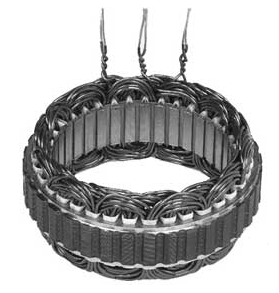
\includegraphics[scale=1]		{figuras/estator_alternador.png}
	\caption{Estator do alternador}
	\label{estator-alternador}
\end{figure}


\item [Regulador de Tensão]

O regulador de tensão do alternador é um dispositivo de proteção do mesmo, utilizado com o objetivo de proteger os equipamentos que usam a energia gerada pelo alternador, ou seja, as cargas conectadas a ele. O regulador protege as cargas por meio do controle da tensão produzida em qualquer regime de rotação do alternador, de modo a limitar a tensão para que não haja picos de corrente elétrica. Além disso, o regulador de tensão é usado com o objetivo de impedir que a bateria utilizada no projeto sofra sobrecarga. 

\item [Ponte Retificadora]
\end{description}

\subsubsection{Alternador Utilizado}

O gerador síncrono utilizado neste projeto trata-se de um alternador do automóvel Chevette com corrente nominal de 35 ampères e tensão de 14 volts. A figura \ref{alternador} apresentada abaixo mostra esse alternador.

\begin{figure}[h]
	\centering
	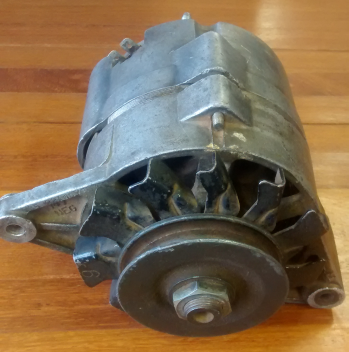
\includegraphics[scale=0.8]		{figuras/alternador.png}
	\caption{Alternador Utilizado}
	\label{alternador}
\end{figure}

\subsection{Cálculo da Corrente de Projeto Necessária}

A corrente de projeto necessária ao atendimento das cargas a ser alimentadas pelo circuito de distribuição da energia elétrica gerada deve ser determinada conforme a equação abaixo:

\begin{equation}
	\mathcal{I}_{proj} = \frac{{P}_{ativa}}{V \times FP}
\end{equation}

Onde:
\begin{description}

\item [Iproj] corrente de projeto em ampère

\item [Pativa] potência ativa total do circuito em watt

\item [V] tensão do circuito em volt

\item [FP] fator de potência total do circuito
\end{description}

Nesse sentido, com base nos dados informados na Tabela xx da seção xx deste relatório, tem-se que a corrente de projeto será igual a xx A.

	Entretanto, a corrente de projeto a ser adotada para o dimensionamento do circuito elétrico será tida como 35 ampères, devido ao fato deste valor ser a capacidade máxima de corrente elétrica que a fonte geradora aqui adotada poderá atingir.
	
	O fato de a corrente de projeto ter sido escolhida acima da necessidade real de nosso projeto é justificado pelo motivo da possibilidade futura de expansão das cargas alimentadas pelo circuito ora projetado, ocorrendo assim a desnecessidade de redimensionamento do sistema elétrico caso novas cargas fossem inseridas no mesmo.

\subsection{Dimensionamento dos Condutores}

O caminho percorrido pela energia elétrica ao longo de um circuito de distribuição deve ser projetado da maneira mais eficiente possível, desde a fonte geradora de corrente elétrica até as cargas terminais, uma vez que parcela daquela energia é dissipada sob a forma térmica devido à resistência elétrica que o fio condutor pelo qual a referida energia se movimenta exerce sobre o fluxo elétrico, restando, assim, prejudicada a eficiência final de distribuição da energia.

Nesse sentido, ao se projetar um circuito elétrico, deve-se procurar minimizar ao máximo possível as perdas de energia ao longo do mesmo e, agindo dessa maneira, terão sido, por consequência, observados aspectos ambientais e conservacionistas ligados ao desperdício de energia. Ademais, deve-se atentar que as perdas oriundas do calor gerado nos condutores de eletricidade reduzirão o nível da tensão disponível no circuito terminal.

Por isso, ao dimensionar os condutores pertinentes ao projeto elétrico ora em estudo, os aspectos acima mencionados foram levados em consideração, a fim de reduzir na prática as supracitadas perdas.
Seguindo esse raciocínio, a escolha dos condutores utilizados neste projeto foi realizada conforme especificações dispostas pela Associação Brasileira de Normas Técnicas (ABNT) na Norma Brasileira número 5410, de 2004 (NBR 5410:2004), cujo teor aborda critérios para o dimensionamento de instalações elétricas de baixa tensão. 
Desse modo, cuidou-se em dimensionar os referidos condutores de acordo com os critérios que visam auxiliar economia de energia, bem como economia de custos financeiros, a fim de atender às necessidades do nosso projeto.

Assim, conforme especificações técnicas daquela NBR, cuidou-se em identificar a "sessão do condutor que reduza o custo da energia desperdiçada, sem incorrer em custos iniciais excessivos de compra e instalação de um cabo", bem como dos dispositivos de proteção necessários, pautando-se pelos seguintes métodos:

\begin{itemize}
	\item Capacidade de condução de corrente
	\item Queda de tensão
	\item Seção mínima
	\item Proteção contra sobrecarga
	\item Proteção contra curto-circuito
	\item Choque elétrico
\end{itemize}

o final dos resultados, em princípio, cada um desses métodos poderá indicar uma seção diferente. Então, segundo a NBR, a seção a ser finalmente adotada consistirá na maior dentre todas as seções obtidas. Vejamos cada um desses métodos.

\subsubsection{Capacidade de Condução de Corrente (artigo 2)}

Segundo (Eletricidade Moderna), o dimensionamento do projeto elétrico seguindo todos os seis critérios mencionados na NBR em comento, têm sua relevância, embora seja compreensível que o critério da capacidade de condução de corrente apresente uma importância que parece ser superior às demais, surgindo como ponto de partida da escolha dos condutores apropriados.

Ainda no entendimento de (Eletricidade Moderna), o critério aqui discutido, de fato, logo após a determinação das cargas existentes no circuito, passando em seguida pelo cálculo da corrente de projeto ($I_{proj}$), tem como etapa seguinte, sendo considerada a primeira em relação ao dimensionamento dos componentes do circuito, a determinação da capacidade de condução de corrente do circuito, determinando assim a seção do condutor que proporcionará nas condições práticas de execução a capacidade de condução de corrente suficiente para a circulação de $I_{proj}$ sem riscos.

Desse modo, em posse do valor de $I_{proj}$, bem como das características de constituição dos condutores, recorreu-se às tabelas que orientam o dimensionamento através do critério em análise, apurando-se a seção do condutor que atenda às necessidades do nosso circuito, vejamos.

Para o caso concreto,\textit{segundo as disposições da NBR}, quanto ao tipo de condutor empregado, ter-se-á condutor isolado (condutor metálico e isolação), sendo o material PVC (cloreto de polivinila). Isso é devido às características de trabalho listadas na Tabela \ref{nbr}, com informações extraídas da NBR.

\begin{table}[h]
\begin{tabular}{| c | p{3cm} | p{3cm} | p{3cm} |}
\hline
Tipo de isolação                & Temperatura máxima para serviço contínuo (condutor) & Temperatura limite de sobrecarga (condutor) & Temperatura limite de curto-circuito (condutor) \\ \hline
Cloreto de polivinila(PVC)      & 70                                                 & 100                                        & 160                                            \\ \hline
Borracha etileno-propileno(EPR) & 90                                                 & 130                                        & 250                                            \\ \hline
Polietileno-reticulado(XLPE)    & 90                                                 & 130                                        & 250                                           
\\ \hline
\end{tabular}
\caption{Características de condutores. Retirado do}
\label{nbr}
\end{table}

Cumpre informar que o motivo da escolha dos condutores com tipo de isolação PVC foi feita devido esse condutor suportar as condições de nosso projeto.

No que tange ao método de instalação a ser utilizado, levou-se em consideração o fato de que este influencia a capacidade de troca térmica entre os condutores e o ambiente circundante, alterando a capacidade de condução de corrente dos condutores. Por isso, através de visita à Tabela xxxx (abaixo) da NBR, foi definido qual método será o mais adequado às condições de nosso projeto, optando-se pelo método de instalação B1.

\begin{figure}[h]
	\centering
	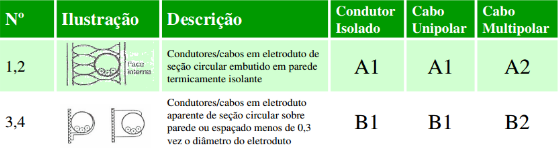
\includegraphics[scale=0.8]		{figuras/nbr.png}
	\caption{NBR - Definição do método}
	\label{alternador}
\end{figure}

Continuando, a NBR diz que a $I_{proj}$ adotada deve ser corrigida por fatores de correção apropriados, os quais são: a) fatores de correção para temperaturas ambientes diferentes; b) correção de resistividade do solo; e c) fator de correção de agrupamento.

Uma vez que as condições de projeto do circuito em discussão não necessitam da utilização desses fatores, seguiu-se o dimensionamento com a $I_{proj}$ anteriormente informada.

	O próximo passo foi determinar o esquema dos condutores, conforme opções listadas na Tabela \ref{metodo-definicao}. Optou-se pelo esquema monofásico a dois condutores.
	
\begin{table}[h]
\centering
\begin{tabular}{| l | p{7cm} |}
\hline
Esquema de condutores vivos do circuito & Número de condutores carregados a ser adotado \\ \hline
Monofásico a dois condutores            & 2                                             \\ \hline
Monofásico a três condutores            & 2                                             \\ \hline
Duas fases sem neutro                   & 2                                             \\ \hline
Duas fases com neutro                   & 3                                             \\ \hline
Trifásico sem neutro                    & 3                                             \\ \hline
Trifásico com neutro                    & 3 ou 4
\\ \hline
\end{tabular}
\caption{Opções de esquema dos condutores}
\label{metodo-definicao}
\end{table}

Após a definição dessas características/parâmetros, o próximo passo foi consultar a Tabela xxx da NBR para efetivar a escolha da seção dos condutores apropriados às condições de projeto, consoante o critério aqui descrito. Portanto, chegou-se à escolha do condutor de seção xxx.

\subsubsection{Queda de Tensão (disposições da UFJF)}

A importância da aplicação desse critério consiste no fato de que as cargas consumidoras de energia elétrica foram projetadas para trabalharem com determinado valor de tensão, aceitando, apenas, reduzida tolerância de não-conformidade com o valor de tensão nominal para o qual a carga foi projetada.
Assim, ao utilizar esse critério, foi levada em consideração a possibilidade dos efeitos anormais que a queda de tensão poderá acarretar às cargas.
 Segundo esse critério, "à medida que a distância entre o medidor de energia e a potência da carga aumenta a queda de tensão ao longo do condutor também aumenta". 
Por isso, baseando-se nesse critério, e com auxílio das características dos condutores adotados neste projeto (PVC, eletroduto não magnético e método de referência B1), somado ao fato de que a NBR informa que em baixa tensão, a queda de tensão nos circuitos terminais não pode ser superior a 4\%, calculou-se a seção dos condutores, veja.

\begin{description}

	\item Cálculo da Queda de Tensão
	%pegar as equaçoes
	
	Com esse resultado, visitou-se a Tabela xxx da fabricante \textit{Pirelli} e constatou-se que para as condições do nosso projeto, a seção do condutor deve ser 6 mm\textsuperscript{2}.
(Lembrar que deve ser atentado ao cálculo da queda de tensão por trecho)

\begin{equation}
	\Delta V = \Delta V_{\frac{V}{A \times km}} \times I_{proj} \times L
\end{equation}
\begin{equation}
	\Delta V_{\frac{V}{A \times km}} = \frac{\Delta V} {I_{proj} \times L}
\end{equation}
\begin{equation}
	\Delta V_{\frac{V}{A \times km}} = \frac{0,04 \times 14}{35 \times 0,002}
\end{equation}
\begin{equation}
	\Delta V_{\frac{V}{A \times km}} = 8 \times \frac{V}{A \times km}
\end{equation}

\end{description}

\subsubsection{Seção Mínima}

As seções mínimas admitidas em qualquer instalação de baixa instalação estão indicadas na Tabela \ref{secoes-minimas}, item xxx da referida Norma. Nesse quesito, traduz-se a tabela, abaixo:

\begin{table}[h]
\begin{tabular}{ |l | p{7cm} | p{5cm} |}
\hline
Instalação                          & Número de condutores carregados a ser adotado           & Seção Mínima para condutores de cobre (mm\textsuperscript{2}) \\ \hline
\multirow{3}{*}{Fixas em geral}     & Circuitos de Iluminação                                 & 1,5                                        \\ \cline{2-3}
                                    & Circuitos de Força                                      & 2,5                                        \\ \cline{2-3}
                                    & Circuitos de sinalização e controle                     & 0,5                                        \\ \hline
\multirow{3}{*}{Ligações flexíveis} & Para um equipamento específico                          & Como especificado na norma do equipamento  \\ \cline{2-3}
                                    & Para qualquer outra aplicação                           & 0,75                                       \\ \cline{2-3} 
                                    & Circuitos a extrabaixa tensão para aplicaçòes especiais &                                           
\\ \hline

\end{tabular}
\caption{Seções Mínimas}
\label{secoes-minimas}
\end{table}

Assim, dentro desse quesito, adotou-se que as ligações de nosso circuito serão do tipo flexíveis, sendo a utilização consistente com circuitos de extra-baixa tensão para aplicações especiais. 

Por isso, levando-se em consideração a Tabela \ref{secoes-minimas}, a seção indicada é 0,75 mm\textsuperscript{2} para os condutores de cobre.

\subsubsection{Outros}

Porém, "como isto significa aumentar o custo do cabo, tende-se a anular a economia conseguida pela melhoria da eficiência na distribuição, sendo que é necessário encontrar-se então um compromisso entre estas duas variáveis".

Por isso, visando economia de energia e uma distribuição de alta eficiência, procurou-se escolher os condutores deste projeto portando-se pela NBR em comento.

\subsection{Dimensionamento dos Dispositivos de Proteção do Circuito}

A proteção é uma ação automática provocada por dispositivos sensíveis a determinadas condições anormais, no sentido de evitar ou limitar danos a um sistema ou equipamento, a proteção também pode ser entendida como uma manobra automática.

A escolha, aplicação e a coordenação seletiva adequadas ao conjunto de componentes que constituem a proteção de um sistema é um dos aspectos mais importantes da instalação elétrica industrial. A função da proteção justamente minimizar os danos ao sistema e seus componentes, sempre que ocorrer uma falha no equipamento, no sistema elétrico ou falha humana.

Os dispositivos de proteção contra correntes de curto-circuito, como: disjuntores e fusíveis. E os dispositivos de proteção contra correntes de sobrecarga, como os relés bimetálicos.
\part{Conclusões}
\chapter[Resultados]{Resultados}

Com a inclusão dos sensores no sistema, obtemos a coleta dos dados que são considerados importantes para as mudanças físicas que irão ocorrer no ambiente virtual, bem como a produção de sensações no usuário de forma que o mesmo tenha um experiência semelhante a andar de bicicleta na rua. Os seguintes dados estão sendo coletados: velocidade e direção a qual o guidão é movimentado.
% e nível da bateria para o sistema de realimentação.

Os dados da velocidade serão apresentados ao atleta para que ele tenha consciência do seu desempenho. O sinal do sensor de direção do guidão fará com que haja uma alteração no ambiente virtual, ou seja, dependendo da angulação do guidão, o usuário terá a sensação de que está fazendo uma curva. Outro dado importante é que quando houver uma subida no percurso do ambiente virtual o usuário terá maior dificuldade ao pedalar, como se realmente estivesse subindo um morro, por exemplo.

Por meio destas características, espera-se simular um ambiente que seja tão próximo quanto possível da realidade de forma a tornar atividades físicas, como o \textit{spinning}, algo menos monótono já que o atleta não se desloca e apresentar dados que possam melhorar seu rendimento. Outro resultado interessante é realizar a comparação do nível de iteratividade do sistema com uma situação real e analisar como o usuário se comporta em ambos os ambientes. Isso é interessante para atletas de alto nível pois simular o percurso de uma prova e ter conhecimento das reações do corpo naquele ambiente é de fundamental importância para um bom desempenho.

Uma das medidas adotadas pela equipe para a produção do produto foi  a busca pela conservação da estrutura original da bicicleta, no intuito que o produto possa ser oferecido como um pacote sem a inclusão da bicicleta, permitindo que com algumas peças e a remoção da roda traseira a bicicleta possa ser adaptada para o uso do produto.


\chapter{Manual do Produto} % (fold)
\label{cha:manual_do_produto}
 
O trecho a seguir descreve o processo recomendado pela equipe para o uso do produto, assim como os cuidados que devem ser tomados com o manuseio.

\section{Modo de Uso} % (fold)
\label{sec:modo_de_uso}

\begin{enumerate}
	\item Verifique se a aplicação já esta em funcionamento com o auxilio da tela secundaria (notebook/monitor).
	\item Posicione-se sobre a bicicleta. Verifique se a mesma se mantem  estável com o seu peso. Para mais informações sobre os valores para qual este produto foi projetado, verificar \autoref{dados_usuario}.
	\item Imerja-se na realidade virtual com o \gls{rift}.
	\item Após o uso do equipamento, remova o \gls{rift} e espere de 15 a 30 segundos antes de tentar desmontar da bicicleta\footnote{Devido a alta imersão, é recomendado um tempo para se acostumar novamente com a realidade antes de realizar movimentos bruscos.}.
\end{enumerate}

\section{Precauções} % (fold)
\label{sec:precau_es}

\begin{description}
	\item [Não tente desmontar da bicicleta utilizando o gls{rift}] $-$ Ao utilizar o \gls{rift}, a imersão proporcionará uma perca da noção de espaço e posição da realidade. Tentar se movimentar na realidade visualizando o ambiente virtual é extremamente desencorajador.
	\item [Não grite] $-$ A imersão no ambiente virtual causa uma perca de contato com a realidade, lembre-se disto antes de tentar se comunicar com aqueles que te assistem.
	\item [Evite balançar muito na bicicleta ou ficar em pé nela] $-$ Apesar de cálculos terem sido feitos no intuito de manter a bicicleta o mais estável possível ao chão, o produto ainda é passível de tombamento quando exposto a determinados momentos angulares.
	\item [Divirta-se] $-$ Mesmo tendo como objetivo apresentar uma alternativa para a pratica de atividades físicas em ambientes fechados, o projeto busca oferecer também entretenimento ao usuário.
	\item [Mantenha o produto] $-$ Evite reajustar os sensores, a altura do guidão ou do banco. Por ser um protótipo, o produto ainda não oferece um amplo grau de personalização. Tentar configurar o equipamento sem o devido conhecimento do produto pode vir a danifica-lo ou  ao comprometimento dos sinais adquiridos para controle do ambiente.
\end{description}

\bookmarksetup{startatroot} 

\postextual

\bibliography{bibliografia} 

\printindex

\glsaddall
\part*{Gloss\'ario}
\providetranslation{Notation (glossaries)}{Notação}
\providetranslation{Description (glossaries)}{Descrição}
\phantomsection
\addcontentsline{toc}{part}{Gloss\'ario}
\glossarystyle{altlisthypergroup}
\printglossary[title= ]

% \newpage
% \phantomsection
% \addcontentsline{toc}{chapter}{Lista de Termos}\label{acrom}
% \printglossary[type=\acronymtype,title=Lista de Termos,toctitle=Lista de Termos]


\end{document}

